\documentclass[11pt,twoside]{article}

\usepackage[margin=1in]{geometry}
\usepackage{amsmath,amssymb,amsthm,mathtools}
\usepackage[inline,shortlabels]{enumitem}
\usepackage{booktabs}
\usepackage{xcolor}
\usepackage{microtype}
\usepackage{needspace}
\usepackage{float}
\usepackage{tikz}
\usetikzlibrary{arrows.meta,calc,positioning}

% Revision date: maintained by scripts/build_lecture_notes.py. Keep this command.
\newcommand{\lecturerevised}{2026-10-09 23:37 UTC-07:00}
\usepackage{eso-pic}
\AddToShipoutPictureBG{%
  \AtPageLowerLeft{%
    \put(\LenToUnit{0.5\paperwidth},\LenToUnit{0.5in}){%
      \makebox(0,0){\normalfont\footnotesize\color{black!60}Last revised: \lecturerevised}%
    }%
  }%
}

\usepackage[square,authoryear]{natbib}
\usepackage[colorlinks=true,linkcolor=blue!60!black,
  urlcolor=blue!60!black,citecolor=blue!60!black]{hyperref}
\usepackage[nameinlink,capitalize]{cleveref}
\crefname{exercise}{Exercise}{Exercises}
\Crefname{exercise}{Exercise}{Exercises}
\hypersetup{pdftitle={Lecture 10: Implicit bias and solution selection},
  pdfauthor={Csaba Szepesvari}}

\usepackage{../exercises/course-exercises}

\usepackage{enotez}
\DeclareInstance{enotez-list}{lecture}{list}{format=\normalsize,number={#1.}}
\setenotez{list-name=Endnotes,list-style=lecture,backref=true}
\crefname{endnote}{Endnote}{Endnotes}
\Crefname{endnote}{Endnote}{Endnotes}

\definecolor{courseblue}{HTML}{17365D}
\newcommand{\E}{\mathbb E}
\newcommand{\I}{\mathbb I}
\newcommand{\one}[1]{\I\{#1\}}
\renewcommand{\P}{\mathbb P}
\newcommand{\R}{\mathbb R}
\newcommand{\suppmark}{\texorpdfstring{\textsuperscript{*}}{*}}
\newcommand{\sign}{\operatorname{sign}}
\newcommand{\range}{\operatorname{range}}
\newcommand{\diag}{\operatorname{diag}}
\newcommand{\argmin}{\operatorname*{arg\,min}}
\newcommand{\argmax}{\operatorname*{arg\,max}}
\makeatletter
\@for\@letter:=A,B,C,D,E,F,G,H,I,J,K,L,M,N,O,P,Q,R,S,T,U,V,W,X,Y,Z\do{%
  \expandafter\edef\csname c\@letter\endcsname{\noexpand\mathcal{\@letter}}}
\makeatother

\newtheorem{theorem}{Theorem}[section]
\newtheorem{proposition}[theorem]{Proposition}
\newtheorem{corollary}[theorem]{Corollary}
\newtheorem{lemma}[theorem]{Lemma}
\theoremstyle{definition}
\newtheorem{definition}[theorem]{Definition}
\newtheorem{example}[theorem]{Example}
\theoremstyle{remark}
\newtheorem{remark}[theorem]{Remark}

\renewcommand{\thepage}{10--\arabic{page}}
\renewcommand{\thesection}{10.\arabic{section}}
\renewcommand{\theequation}{10.\arabic{equation}}
\pagestyle{myheadings}
\markboth{Lecture 10: Implicit bias and solution selection}
{Lecture 10: Implicit bias and solution selection}

\begin{document}

\begin{center}
\fcolorbox{courseblue}{white}{%
\begin{minipage}{0.92\textwidth}
\vspace{1mm}
\textbf{CMPUT 654: Mathematical Foundations of Modern AI Systems}
\hfill Fall 2026

\vspace{3mm}
\begin{center}
{\Large\bfseries Lecture 10: Implicit bias and solution selection}

\vspace{1mm}
October 6, 2026
\end{center}

\vspace{2mm}
\textit{Lecturer: Csaba Szepesv\'ari}
\hfill
\textit{Note prepared by: Csaba Szepesv\'ari}
\vspace{1mm}
\end{minipage}}
\end{center}

\noindent\textbf{Reading guide.}
The empirical objective need not determine one predictor. This lecture asks
what an optimization method selects among the resulting possibilities. The
main text follows the development in class. We first distinguish
non-uniqueness of parameters
from non-uniqueness of the represented model. We then pay a debt from
Lecture~9 by proving that zero-initialized gradient descent selects the
minimum-Euclidean-norm least-squares interpolant. The central case is linear
logistic classification on separable data: gradient descent and signed
gradient descent select different max-margin directions, and either direction
can have smaller population classification risk. We prove the continuous-time
steepest-descent result used to explain this selection, discuss the two regimes
of Adam, and finish the main exposition with the distinction between constant
and decreasing stepsizes under different sources of gradient noise. Material
not reached in class is marked with $\suppmark$. The supplementary material
treats early stopping as a spectral filter, the construction of
\citet{wilson2017}, noise-induced
selection in neural networks, and parameter-space flatness. The prerequisites
are linear algebra, least squares, and elementary probability.

\section{When empirical fit does not determine the predictor}
\label{sec:setup}

Let $f_w$ denote the predictor represented by a parameter vector $w$, and let
$L_n(w)$ be its empirical training loss. If $L_n$ has many minimizers, two
different kinds of non-uniqueness must be separated.

\begin{definition}[Parameter and model non-uniqueness]
\label{def:two-nonuniqueness}
There is \emph{parameter-space non-uniqueness} when distinct parameters
$w\ne w'$ both minimize the empirical loss. There is \emph{model
non-uniqueness} when empirical minimizers represent predictors that differ on
some input: $f_w\ne f_{w'}$.
\end{definition}

Parameter-space non-uniqueness need not produce model non-uniqueness. In a
neural network, permuting hidden units can leave the represented function
unchanged. For a positively homogeneous unit, the rescaling
\[
 a[b^\top x]_+=\frac ac[(cb)^\top x]_+,
 \qquad c>0,
\]
also changes the parameters without changing the predictor. Such parameter
symmetries matter when discussing optimization paths or parameter-space
curvature, but the symmetries do not by themselves change a prediction. The
statistical issue in this lecture is model non-uniqueness: different empirical
minimizers or limiting directions can extrapolate differently beyond the
training sample.

Overparameterization makes underdetermination common. In linear regression,
the data can constrain only the component of a parameter in the span of the
training inputs. In a neural network, there may be many more degrees of
freedom than empirical constraints. Once the empirical objective leaves a
choice, the optimization procedure can do more than merely reduce the
objective: the procedure's initialization, update rule, and stopping time can
select among the empirically equivalent alternatives.

\begin{definition}[Explicit regularization and implicit bias]
\label{def:regularization-bias}
A \emph{regularizer} is an auxiliary parameter- or predictor-dependent
criterion $\Omega(w)$ used to prefer some fits to others. The preference is
\emph{explicit} when training minimizes, for example,
\[
 L_n(w)+\lambda\Omega(w)
 \qquad\text{or imposes}\qquad \Omega(w)\le r.
\]
The \emph{implicit bias} of an optimization procedure is a preference induced
by its initialization, update geometry, or stopping rule while the model and
empirical objective are held fixed. In this lecture, \emph{algorithmic bias}
refers to this optimizer-induced selection.
\end{definition}

The classical origin of regularization is statistical. In a rich
nonparametric class, exact empirical fitting can reproduce noise or behave
irregularly between observed inputs. One therefore adds a complexity or
roughness penalty, such as
\begin{equation}
 \widehat f_\lambda\in\argmin_{f\in\mathcal F}
 \left\{\frac1n\sum_{i=1}^n\bigl(Y_i-f(X_i)\bigr)^2
       +\lambda J(f)\right\}.
 \label{eq:nonparametric-regularization}
\end{equation}
The strength $\lambda$ may be chosen from the data, and in asymptotic analyses
$\lambda$ commonly decreases with $n$. Implicit bias is surprising because a
choice of optimizer can create a preference resembling regularization without
adding the term $\lambda J$ to the empirical objective.

Population performance remains the criterion for deciding whether the
preference is useful. If the training sample is random with law $P$, write
\[
 R_P(w)=\E_P[\ell_{\rm eval}(w;\,\cdot)]
\]
for the population risk. The evaluation loss may differ from the empirical
training loss. When the optimizer itself adds bias, the main question is
whether the induced bias decreases the population risk. Computational
efficiency---using less computation to reach a given empirical loss, or
reaching a smaller empirical loss within a fixed computational budget---also
matters, but downstream performance is the criterion studied here.

We analyze the relation between optimizer-induced bias and population risk in
two linear cases.

\section{Least squares: initialization determines the invisible component}
\label{sec:least-squares}

Consider linear least squares when the number of parameters is greater
than the number of datapoints. The minimizer of the loss is not unique:
Any interpolating solution leads to zero (minimum) loss, and there are
many such solutions.

Lecture~9 motivated minimum-norm interpolation by stating that gradient
descent has an algorithmic bias toward a minimum-norm solution. Lecture~9
also studied the downstream consequences and found that the usefulness of
this bias depends on the choice and scaling of features. We now prove the
selection claim about gradient descent.

To prove this selection claim, fix $x_1,\ldots,x_n\in\R^d$ and
$y_1,\ldots,y_n\in\R$, and define the
\emph{data span}
\[
 \cR=\operatorname{span}\{x_1,\ldots,x_n\}\subseteq\R^d\,.
\]
The data span $\cR$ is a linear subspace of $\R^d$. When there are more
parameters than datapoints ($d>n$), i.e., in the overparametrized regime,
$\cR$ is a nontrivial subspace of $\R^d$; that is, $\cR\ne\R^d$.
The orthogonal complement of the data span is
\[
 \cR^\perp=\{v\in\R^d:\langle v,x_i\rangle=0
                       \text{ for every }i\in[n]\}.
\]
Predictions take the form $x \mapsto \langle x, w \rangle$ where $w\in \R^d$ is
a model parameter. Let $f_w(x) = \langle x, w \rangle$.
The data cannot distinguish $w$ from $w+v$ when $v\in\cR^\perp$ in the sense
that $f_w(x_i)= f_{w+v}(x_i)$ for all $i\in [n]$ for any $w\in \R^d$ and $v\in \cR^\perp$.

Consider
\begin{equation}
 L_n(w)=\frac12\sum_{i=1}^n
          \bigl(\langle w,x_i\rangle-y_i\bigr)^2.
 \label{eq:least-squares-loss}
\end{equation}
The gradient equation
\begin{equation}
 \nabla L_n(w)
 =\sum_{i=1}^n\bigl(\langle w,x_i\rangle-y_i\bigr)x_i=0
 \label{eq:normal-equation-sum}
\end{equation}
is called the \emph{normal equation}. To write it in matrix form, let
$\mathbf X\in\R^{n\times d}$ have row $i$ equal to $x_i^\top$, and let
$y=(y_1,\ldots,y_n)^\top$. Then
\[
 \nabla L_n(w)=\mathbf X^\top(\mathbf Xw-y).
\]

Assume
\begin{equation}
 \dim(\cR)=n.
 \label{eq:independent-training-vectors}
\end{equation}
The rank theorem says that condition
\cref{eq:independent-training-vectors} is equivalent to
$\mathbf X\mathbf X^\top$ being nonsingular. The rank theorem also implies
that
$\mathbf X:\R^d\to\R^n$ is onto. Consequently, arbitrary responses
$y\in\R^n$ can be interpolated. Moreover, $\mathbf X^\top$ is one-to-one,
so the normal equation is equivalent to
\begin{equation}
 \mathbf Xw=y.
 \label{eq:least-squares-interpolation}
\end{equation}
Thus every minimizer interpolates and has loss zero. Conversely, every
interpolant has loss zero and is therefore a minimizer.

Define
\begin{equation}
 w^\star=\mathbf X^\top
          (\mathbf X\mathbf X^\top)^{-1}y.
 \label{eq:least-squares-minimum-norm}
\end{equation}
Substitution gives $\mathbf Xw^\star=y$, and $w^\star\in\cR$ because $w^\star$ is
a linear combination of the $x_i$.

\begin{proposition}[Initialization determines the least-squares interpolant]
\label{prop:ls-selection}
Every minimizer of \cref{eq:least-squares-loss} has the unique form
\[
 w^\star+v,
 \qquad v\in\cR^\perp.
\]
The vector $w^\star$ is the unique minimum-Euclidean-norm minimizer.
Furthermore, consider gradient descent
\begin{equation}
 w_{t+1}=w_t-
 \eta\sum_{i=1}^n
 \bigl(\langle w_t,x_i\rangle-y_i\bigr)x_i,
 \qquad
 0<\eta<\frac{2}{\|\mathbf X\|_{\rm op}^2}.
 \label{eq:least-squares-gd}
\end{equation}
If $v_0$ is the orthogonal projection of $w_0$ onto $\cR^\perp$, then
\[
 w_t\longrightarrow w^\star+v_0.
\]
In particular, $w_0=0$ selects $w^\star$.
\end{proposition}

\begin{proof}
If $w$ is a minimizer, then \cref{eq:least-squares-interpolation} and
$\mathbf Xw^\star=y$ give
\[
 \langle w-w^\star,x_i\rangle=0
 \qquad(i\in[n]).
\]
Hence $w-w^\star\in\cR^\perp$. Conversely,
$\mathbf X(w^\star+v)=y$ for every $v\in\cR^\perp$, proving the claimed
description of all minimizers. Since $w^\star\in\cR$ and
$v\in\cR^\perp$, the Pythagorean theorem gives
\[
 \|w^\star+v\|_2^2=\|w^\star\|_2^2+\|v\|_2^2.
\]
Therefore $w^\star$ is the unique minimum-norm minimizer.

Every increment $w_{t+1}-w_t$ in \cref{eq:least-squares-gd} is a linear
combination of the $x_i$ and hence belongs to $\cR$. The component of $w_t$ in
$\cR^\perp$ therefore remains equal to $v_0$. Write $w_t=r_t+v_0$ with
$r_t\in\cR$. Since $\mathbf Xv_0=0$ and $\mathbf Xw^\star=y$,
\[
 r_{t+1}-w^\star
 =\bigl(I-\eta\mathbf X^\top\mathbf X\bigr)(r_t-w^\star).
\]
The restriction of $\mathbf X^\top\mathbf X$ to $\cR$ is positive
definite. The eigenvalues of this restriction lie in
$(0,\|\mathbf X\|_{\rm op}^2]$, so the stepsize assumption makes the last
linear map a strict contraction on every eigendirection in $\cR$. Thus
$r_t\to w^\star$ and $w_t\to w^\star+v_0$.
\end{proof}

The argument separates what the data determine from what initialization
supplies. The rank assumption guarantees that the observed responses can be
fit. The orthogonal decomposition says that the data constrain the component
in $\cR$ and cannot see the component in $\cR^\perp$. Zero initialization
sets that invisible component to zero, and gradients cannot create it.
\Cref{ex:l10-least-squares-selection} asks you to reconstruct the argument
and to show explicitly why another initialization need not select the
minimum-norm solution.

\section{Logistic classification on separable data}
\label{sec:max-margin}

Lecture~1 introduced logits and the softmax map that converts an LLM's output
scores into next-token probabilities. Training uses token log loss, whereas
many deployment criteria record a discrete event such as whether the final
answer is correct. The binary linear logistic model is the smallest model
that retains the distinction between training and deployment losses.
The binary model lets us study how a smooth probabilistic training objective
can produce a sharp discrete prediction and how the optimizer can affect that
prediction on unseen inputs. The binary linear model does not describe the
full computation performed by a transformer.

The linear score
\[
 s_w(x)=\langle w,x\rangle
\]
is a \emph{logit}. The sigmoid function and the resulting conditional
probability model are
\[
 \sigma(s)=\frac1{1+e^{-s}},
 \qquad
 q_w(y\mid x)=\sigma\bigl(ys_w(x)\bigr),
 \qquad y\in\{-1,1\}.
\]
The identity $\sigma(s)+\sigma(-s)=1$ makes $q_w(\cdot\mid x)$ a probability
mass function, and
\[
 \log\frac{q_w(1\mid x)}{q_w(-1\mid x)}=s_w(x).
\]
Thus the log-odds are linear in $x$. The log-odds identity explains the name
\emph{logistic regression} in two parts. ``Logistic'' refers to the logistic
link $p=\sigma(s)$ that converts a score into a probability. ``Regression''
refers to modeling a conditional mean as a function of the input. Indeed, for
$B=(Y+1)/2\in\{0,1\}$,
\[
 \E[B\mid X=x]=\P(Y=1\mid X=x)
 \approx q_w(1\mid x)=\sigma(\langle w,x\rangle).
\]
Thus logistic regression models the conditional mean of a binary response,
equivalently its success probability, through linear log-odds. Thresholding
that fitted probability at $1/2$ turns the model into a classifier.

The negative log-likelihood of a labeled example is
\[
 -\log q_w(y\mid x)=\log\bigl(1+e^{-ys_w(x)}\bigr).
\]
Fix training examples
$(x_1,y_1),\ldots,(x_n,y_n)\in\R^d\times\{-1,1\}$. Training minimizes the
empirical logistic loss
\begin{equation}
 L_n(w)=\frac1n\sum_{i=1}^n
 \log\bigl(1+\exp(-y_i\langle w,x_i\rangle)\bigr).
 \label{eq:empirical-logistic}
\end{equation}
At deployment, the predicted label is $h_w(x)=\sign(s_w(x))$, with
$\sign(0)=1$. If $(X,Y)$ has law $P$, the population classification risk is
\begin{equation}
 R_P(w)=\P\bigl(h_w(X)\ne Y\bigr),
 \label{eq:population-risk}
\end{equation}
The smooth logistic loss is therefore a \emph{surrogate loss}: a tractable
training loss used in place of the deployment loss
$\one{h_w(x)\ne y}$. Log loss is a \emph{strictly proper scoring rule}: for
each input $x$, its conditional expectation is uniquely minimized by
predicting the true value of $\P(Y=1\mid X=x)$. This proper-scoring property
is why probability
fitting, rather than classification alone, explains the word ``regression.''
Lecture~1 introduced the binary logit as log-odds, while Lecture~3 introduced
sigmoid probabilities and log-loss fitting. The following review combines
those ideas
for a linear score. \Cref{ex:l10-logistic-log-loss} asks you to derive the
identities and use them to explain the name logistic regression.

More generally, a \emph{margin loss} has the form $\ell(m)$, where
$m=ys_w(x)$ is the signed margin. Common examples are
\[
 \ell_{\rm log}(m)=\log(1+e^{-m}),
 \qquad
 \ell_{\rm exp}(m)=e^{-m},
 \qquad
 \ell_{\rm hinge}(m)=(1-m)_+.
\]
These losses decrease as the signed margin increases, but the name
``margin loss'' alone does not determine a probability model or an implicit
bias. The tail of $\ell$ and the update geometry both affect the limiting
direction. We analyze logistic loss below.

Write
\[
 z_i=y_ix_i
\]
for the \emph{signed feature vector}. The loss depends on $(x_i,y_i)$ only
through $z_i$:
\[
 \log\bigl(1+e^{-y_i\langle w,x_i\rangle}\bigr)
 =\log\bigl(1+e^{-\langle w,z_i\rangle}\bigr).
\]
In particular, $(x_i,y_i)$ and $(-x_i,-y_i)$ have exactly the same effect on
the empirical loss. A finite training sample is
\emph{linearly separable} if some $w$ satisfies
\begin{equation}
 \langle w,z_i\rangle>0
 \qquad\text{for every }i\in[n].
 \label{eq:separable}
\end{equation}
The term ``linearly separable'' here refers to the observed sample, not
automatically to the population law. On a separable sample, scaling such a $w$ drives
\cref{eq:empirical-logistic} to zero. No finite vector attains zero, so the
relevant selected object is a direction.

\begin{figure}[H]
\centering
\definecolor{tabblue}{HTML}{1F77B4}
\definecolor{taborange}{HTML}{FF7F0E}
\newcommand{\ltenseparabledata}{%
  \foreach \a/\b in {-1.4/0.9,-0.9/1.4,-0.6/0.5,-1.5/1.5,0.2/1.6,0.5/0.8,0.9/0.5,1.0/1.3,1.5/1.2,0.6/1.8,-0.5/1.0}
    \fill[tabblue] (\a,\b) circle (1.5pt);
  \foreach \a/\b in {-1.3/-1.0,-0.8/-0.7,-0.4/-1.2,0.1/-0.7,0.4/-1.5,0.8/-0.9,1.3/-0.6,-1.5/-1.4,-0.9/-1.7,1.4/-1.2}
    \fill[taborange] (\a,\b) circle (1.5pt);
}
\hfill
\begin{tikzpicture}[scale=1.15,>=stealth]
  \draw[->,black!45] (-2.4,0) -- (2.4,0);
  \draw[->,black!45] (0,-2.4) -- (0,2.4);
  \begin{scope}[rotate=20]
    \draw[thick] (-2.3,0) -- (2.3,0);
    \ltenseparabledata
    \draw[->,thick] (0,0) -- (0,1.1) node[left] {$w$};
  \end{scope}
\end{tikzpicture}
\hfill
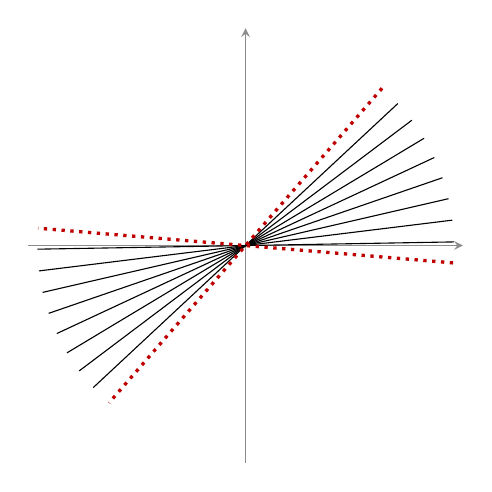
\begin{tikzpicture}[scale=1.15,>=stealth]
  \draw[->,black!45] (-2.4,0) -- (2.4,0);
  \draw[->,black!45] (0,-2.4) -- (0,2.4);
  \begin{scope}[rotate=20]
    \foreach \t in {-19,-13,-7,-1,5,11,17,23}
      \draw[thin] (\t:2.3) -- (\t+180:2.3);
    \draw[red!75!black,dotted,line width=1.2pt]
      (29.05:2.3) -- (209.05:2.3);
    \draw[red!75!black,dotted,line width=1.2pt]
      (-24.78:2.3) -- (155.22:2.3);
    \ltenseparabledata
  \end{scope}
\end{tikzpicture}
\hfill\mbox{}
\caption{One separating hyperplane (left) and several of the separating
hyperplanes for the same sample (right). The dotted boundary lines touch a
data point and therefore do not strictly separate the sample.}
\label{fig:separable-data}
\end{figure}

Separability is an idealized property of the data at hand. A high-dimensional
finite sample can be separable even when the population contains label noise.
The max-margin asymptotics below describe training only while the separable
model remains appropriate; they should not be applied automatically to a
nonseparable or continually changing dataset.

Two discrete algorithms will be compared. With
$g_t=\nabla L_n(w_t)$, ordinary gradient descent and signed gradient descent
use
\begin{align}
 w_{t+1}&=w_t-\eta_t g_t,
 \label{eq:logistic-gd}\\
 w_{t+1}&=w_t-\eta_t\sign(g_t),
 \label{eq:logistic-signgd}
\end{align}
respectively. The sign is applied coordinatewise. Both methods can drive the
empirical loss toward zero, but they need not approach the same direction.

For $p\in[1,\infty]$, define the \emph{normalized empirical margin}
\[
 \gamma_p(w)=\frac{\min_{i\in[n]}\langle w,z_i\rangle}{\|w\|_p},
 \qquad w\ne0.
\]
The normalized margin $\gamma_p(w)$ is unchanged when $w$ is multiplied by a
positive scalar, so $\gamma_p(w)$ depends only on the direction of the
parameter vector $w$.
The norm used for normalization is a choice. At this point there is no reason
internal to logistic loss to select
$p=2$, $p=\infty$, or another value. We keep $p$ explicit because two choices
will arise naturally from two optimization methods.

Maximizing $\gamma_p$ is equivalent, after rescaling the smallest margin to
one, to the hard-margin problem
\begin{equation}
 \min_w\|w\|_p
 \quad\text{subject to}\quad
 \langle w,z_i\rangle\ge1\quad(i\in[n]).
 \label{eq:p-margin}
\end{equation}
Thus varying $p$ in \cref{eq:p-margin} gives a family of norm-constrained
optimization problems. A solution of each problem determines a separating
direction, and the optimizer can select among these directions.

\begin{theorem}[Gradient and signed gradient descent select norm-dependent margins]
\label{thm:discrete-margin-selection}
Fix a linearly separable sample.
\begin{enumerate}[(a),leftmargin=*]
\item For a sufficiently small constant stepsize, the gradient-descent
iterates in \cref{eq:logistic-gd} satisfy
$\gamma_2(w_t)\longrightarrow\gamma_2^\star$.
If the maximum-$\ell_2$-margin direction is unique, then the normalized
iterates converge to that direction.
\item Suppose the signed-gradient stepsizes in
\cref{eq:logistic-signgd} are positive and nonincreasing, with
 $\eta_t\longrightarrow0$,
 $
 \sum_{t=0}^\infty\eta_t=\infty$.
Then
\[
 \gamma_\infty(w_t)\longrightarrow\gamma_\infty^\star.
\]
If the maximum-$\ell_\infty$-margin direction is unique, then the normalized
iterates converge to that direction.
\end{enumerate}
\end{theorem}

The stepsize assumptions are algorithm-specific. Gradient descent scales its
step by the magnitude of the gradient, whereas signed descent takes a unit
$\ell_\infty$ direction before applying $\eta_t$. The theorem says that
gradient descent prefers Euclidean geometry, while signed descent prefers
max-norm geometry. The theorem does not determine which preference has
smaller population risk. \Cref{sec:two-dimensional,sec:amplification} give
distributions on
which either ordering occurs.

The conditions on $\eta_t$ are not cosmetic. On separable data the parameter
norm must diverge, while the logistic gradient becomes exponentially small in
the margins. A stepsize that decreases too quickly can leave insufficient
cumulative movement. Conversely, more aggressive and even increasing
stepsizes are possible for some algorithms and losses, but require a separate
analysis of the discretization error.

\section{Why steepest descent selects a margin geometry}
\label{sec:steepest-flow}

Why do the two algorithms in \cref{thm:discrete-margin-selection} select
different max-margin geometries? They measure the size of an update in
different norms.
The steepest-descent formulation makes the difference between the two update
geometries explicit.

To see the connection before stating the theorem, let $q$ be the H\"older
conjugate of $p$, so $1/p+1/q=1$, and let $g\ne0$ be a gradient. A
\emph{unit steepest-descent direction} measured in $\|\cdot\|_p$ is
\begin{equation}
 s_p(g)\in\argmin_{\|v\|_p=1}\langle g,v\rangle.
 \label{eq:steepest-direction}
\end{equation}
Thus one unit of movement is charged according to the $\ell_p$ norm.
H\"older's inequality and \cref{eq:steepest-direction} give
\begin{equation}
 \|s_p(g)\|_p=1,
 \qquad
 \langle-g,s_p(g)\rangle=\|g\|_q.
 \label{eq:steepest-identities}
\end{equation}

\begin{figure}[H]
\centering
\hfill
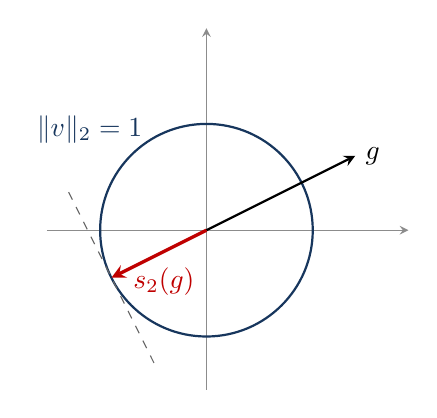
\begin{tikzpicture}[scale=1.35,>=stealth]
  \draw[->,black!45] (-1.5,0) -- (1.9,0);
  \draw[->,black!45] (0,-1.5) -- (0,1.9);
  \draw[thick,courseblue] (0,0) circle (1);
  \draw[dashed,black!60] (-1.296,0.358) -- (-0.492,-1.252);
  \draw[->,thick] (0,0) -- (1.4,0.7) node[right] {$g$};
  \draw[->,very thick,red!75!black] (0,0) -- (-0.894,-0.447);
  \node[red!75!black] at (-0.4,-0.48) {$s_2(g)$};
  \node[courseblue] at (-1.1,0.95) {$\|v\|_2=1$};
\end{tikzpicture}
\hfill
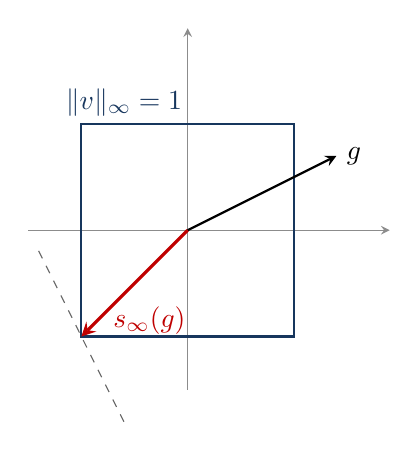
\begin{tikzpicture}[scale=1.35,>=stealth]
  \draw[->,black!45] (-1.5,0) -- (1.9,0);
  \draw[->,black!45] (0,-1.5) -- (0,1.9);
  \draw[thick,courseblue] (-1,-1) rectangle (1,1);
  \draw[dashed,black!60] (-1.402,-0.195) -- (-0.598,-1.805);
  \draw[->,thick] (0,0) -- (1.4,0.7) node[right] {$g$};
  \draw[->,very thick,red!75!black] (0,0) -- (-1,-1);
  \node[red!75!black] at (-0.36,-0.85) {$s_\infty(g)$};
  \node[courseblue] at (-0.6,1.2) {$\|v\|_\infty=1$};
\end{tikzpicture}
\hfill\mbox{}
\caption{The unit steepest directions for the Euclidean norm (left) and the
max norm (right). In each panel, the dashed level set of
$v\mapsto\langle-g,v\rangle$ supports the unit ball at $s_p(g)$.}
\label{fig:steepest-directions}
\end{figure}

The two cases in the figure are
\[
 s_2(g)=-\frac{g}{\|g\|_2},
 \qquad
 s_\infty(g)=-\sign(g).
\]
These formulas identify the directions followed by gradient descent and signed
gradient descent, but not their step lengths. A second standard convention
defines the \emph{scaled steepest-descent vector}
\begin{equation}
 d_p(g)\in\argmin_v
 \left\{\langle g,v\rangle+\frac12\|v\|_p^2\right\}.
 \label{eq:scaled-steepest-vector}
\end{equation}
For compatible choices of minimizers,
\[
 d_p(g)=\|g\|_q s_p(g),
 \qquad d_2(g)=-g,
 \qquad d_\infty(g)=-\|g\|_1\sign(g).
\]
Thus ordinary gradient descent is exactly scaled Euclidean steepest descent.
Signed gradient descent is exactly unit max-norm steepest descent; signed
descent follows the same direction as scaled max-norm steepest descent but
uses a different step length.

The distinction between unit and scaled steepest descent determines which
stepsize theorem applies. If
\[
 w_{t+1}=w_t+\alpha_t s_p(g_t)
 \quad\text{and}\quad
 w_{t+1}=w_t+\eta_t d_p(g_t),
\]
then the updates agree precisely when
\begin{equation}
 \alpha_t=\eta_t\|g_t\|_q.
 \label{eq:unit-scaled-steps}
\end{equation}
For signed descent, the unit-direction lengths in
\cref{thm:discrete-margin-selection} decrease to zero but have infinite sum.
For ordinary gradient descent with a small constant multiplier, the actual
unit-direction length is $\alpha_t=\eta\|g_t\|_2$ and shrinks with the
gradient. General scaled steepest-descent results impose conditions on
$\eta_t$; pure signed descent corresponds instead to the scaled multiplier
$\eta_t/\|g_t\|_1$, which need not remain bounded. Hence agreement of
directions is not enough to transfer a discrete-time theorem. Both parts of
\cref{thm:discrete-margin-selection} fit the useful pattern that the actual
movement tends to zero but has infinite cumulative length.

Let
\[
 \gamma_p^\star=\max_{\|u\|_p\le1}
                 \min_{i\in[n]}\langle u,z_i\rangle.
\]
On separable data, $\gamma_p^\star>0$. For continuous time, let
\[
 g(t)=\nabla L_n(w(t))
\]
and consider the unit-speed steepest-descent flow
\begin{equation}
 \dot w(t)=s_p(g(t))
 =s_p\bigl(\nabla L_n(w(t))\bigr),
 \qquad w(0)=w_0.
 \label{eq:unit-steepest-flow}
\end{equation}
Here $w:[0,\infty)\to\R^d$ is a function of time and
$\dot w(t)=\frac{d}{dt}w(t)$; \cref{eq:unit-steepest-flow} is an ordinary
differential equation relating the trajectory $w$ to its derivative. Thus
$\|\dot w(t)\|_p=1$. Positive rescaling of the right-hand side gives the same
continuous trajectory with a different time parameterization.

\begin{theorem}[Steepest-descent flow maximizes the corresponding margin]
\label{thm:margin-geometry}
For the flow in \cref{eq:unit-steepest-flow} on a linearly separable sample,
\[
 \gamma_p(w(t))\longrightarrow\gamma_p^\star.
\]
Every directional limit point $u$ satisfies
$\min_i\langle u,z_i\rangle=\gamma_p^\star$ and $\|u\|_p=1$; consequently,
$u/\gamma_p^\star$ solves \cref{eq:p-margin}. If the maximum-margin direction
is unique, then
$w(t)/\|w(t)\|_p$ converges to that direction.
\end{theorem}

\begin{proof}
Along the flow, write $w=w(t)$, $g=\nabla L_n(w)$, and $L=L_n(w)$, and
suppress the dependence on $t$. A preliminary calculation, asked for in
\cref{ex:l10-flow-escape}, gives
\begin{equation}
 L\longrightarrow0, \qquad \|w\|_p\longrightarrow\infty.
 \label{eq:flow-escape-facts}
\end{equation}
We prove the asymptotic comparison
\begin{equation}
 -\frac{d}{dt}\log L \ge (\gamma_p^\star-\varepsilon)\frac{d}{dt}\|w\|_p
 \label{eq:loss-faster-than-norm}
\end{equation}
for every $\varepsilon\in(0,\gamma_p^\star)$ and all sufficiently large $t$.

Suppose first that \cref{eq:loss-faster-than-norm} holds. Integrating the
inequality from a sufficiently large fixed time $t_0$ to $T$ and using
\cref{eq:flow-escape-facts} gives
\[
 \liminf_{T\to\infty}\frac{-\log L_n(w(T))}{\|w(T)\|_p}\ge\gamma_p^\star-\varepsilon.
\]
\Cref{ex:l10-flow-proof-details} asks you to write out this integration and
the remaining finite-sum details. In particular, the finite sum defining
$L_n$ and $L\to0$ give
\[
 -\log L_n(w)=\min_{i\in[n]}\langle w,z_i\rangle+O(1).
\]
After sending $\varepsilon\downarrow0$ and using $\|w\|_p\to\infty$,
\[
 \liminf_{t\to\infty}\gamma_p(w(t))\ge\gamma_p^\star.
\]
The reverse inequality holds at every time by the definition of
$\gamma_p^\star$. To finish the proof, it remains only to establish
\cref{eq:loss-faster-than-norm}.

Choose $u_p^\star$ with $\|u_p^\star\|_p=1$ and
$\min_i\langle u_p^\star,z_i\rangle=\gamma_p^\star$. The flow definition and
\cref{eq:steepest-identities} give
\begin{equation}
 -\dot L=-\langle g,\dot w\rangle=-\langle g,s_p(g)\rangle=\|g\|_q.
 \label{eq:flow-loss-derivative}
\end{equation}
Moreover, letting
$a_i=\frac1{n(1+e^{\langle w,z_i\rangle})}$, $i\in [n]$, we calculate
\begin{equation}
 -g=-\nabla L_n(w)=\sum_{i=1}^n a_i z_i.
 \label{eq:logistic-gradient-combination}
\end{equation}
Consequently, norm duality and the definition of $u_p^\star$ give
\begin{equation}
 \|g\|_q\ge\langle-g,u_p^\star\rangle=\sum_{i=1}^n a_i\langle z_i,u_p^\star\rangle\ge\gamma_p^\star A\,,
 \label{eq:gradient-margin-lower-bound}
\end{equation}
where we defined $A= \sum_i a_i$.
Because $L\to0$ and its finitely many summands are nonnegative, every margin
tends to infinity. Hence
$\frac{1}{1+e^m}\sim e^{-m}$ and $\log(1+e^{-m})\sim e^{-m}$
imply $A/L\to1$. Therefore, for all sufficiently large $t$,
\begin{equation}
 -\frac{d}{dt}\log L=\frac{-\dot L}{L}=\frac{\|g\|_q}{L}\ge\gamma_p^\star\frac{A}{L}\ge\gamma_p^\star-\varepsilon.
 \label{eq:log-loss-rate}
\end{equation}
Finally, the reverse triangle inequality gives, for $h>0$,
\[
 \frac{\|w(t+h)\|_p-\|w(t)\|_p}{h}\le\frac{\|w(t+h)-w(t)\|_p}{h}.
\]
Letting $h\downarrow0$ and using $\dot w=s_p(g)$ yields, for almost every
$t$,
\begin{equation}
 \frac{d}{dt}\|w\|_p\le\|\dot w\|_p=1.
 \label{eq:norm-growth-at-most-one}
\end{equation}
Combining \cref{eq:log-loss-rate,eq:norm-growth-at-most-one} proves
\cref{eq:loss-faster-than-norm}. The margin conclusion follows from the first
part of the argument. The statement about directional limit points follows
from the equivalent norm-minimization formulation in \cref{eq:p-margin}.
\end{proof}

The theorem proves the continuous-time statement. The discrete result in
\cref{thm:discrete-margin-selection} requires a separate one-step loss bound,
and its assumptions depend on whether the update uses $s_p(g_t)$ or
$d_p(g_t)$. \Cref{ex:l10-discrete-steepest} asks you to carry out this
comparison for a scaled update and to translate between the two stepsize
conventions using \cref{eq:unit-scaled-steps}.

Ordinary gradient descent therefore constructs a Euclidean max-margin
direction, while signed descent constructs a max-norm direction. Both fit the
observed labels, but they can assign different signs to unobserved inputs.
Population risk determines which extrapolation is useful. The next section
makes this dependence exact.

\section{A two-dimensional reversal}
\label{sec:two-dimensional}

Optimization has now selected a direction. Does the selected direction affect
population prediction? In an overparameterized problem, the training sample
can constrain the score on observed inputs without determining the signs
assigned to
unseen inputs. The answer is therefore yes: two directions can classify the
same training sample perfectly and have different population risks. We begin
with the smallest exact example. The example also shows that either direction
can be
better, depending on the population law. \Cref{sec:amplification} then turns
the order-$1/n$ difference into a constant one.

Suppose the training sample contains only the signed vector
\[
 z_0=(2,1)^\top.
\]
The hard-margin constraint is $\langle w,z_0\rangle\ge1$.

\Needspace{13\baselineskip}
\begin{proposition}[One observation produces two separators]
\label{prop:two-selectors}
For the constraint $\langle w,z_0\rangle\ge1$, the minimum-$\ell_2$ and
minimum-$\ell_\infty$ solutions are, respectively,
\[
 w_2=\left(\frac25,\frac15\right)^\top,
 \qquad
 w_\infty=\left(\frac13,\frac13\right)^\top.
\]
For
\[
 u=(1,-3/2)^\top,
 \qquad
 v=(-1,3/2)^\top,
\]
their signed scores have opposite signs:
\[
 \langle w_2,u\rangle>0>\langle w_\infty,u\rangle,
 \qquad
 \langle w_\infty,v\rangle>0>\langle w_2,v\rangle.
\]
\end{proposition}

\begin{proof}
The Euclidean solution is the projection of zero onto the constraint
boundary, so $w_2=z_0/\|z_0\|_2^2=(2/5,1/5)^\top$. H\"older's inequality
gives $1\le\langle w,z_0\rangle\le3\|w\|_\infty$, with equality at
$w_\infty=(1/3,1/3)^\top$. Direct calculation gives
\[
 \langle w_2,u\rangle=\frac1{10},\quad
 \langle w_\infty,u\rangle=-\frac16,
 \quad
 \langle w_2,v\rangle=-\frac1{10},\quad
 \langle w_\infty,v\rangle=\frac16.
\]
\end{proof}

\begin{figure}[H]
\centering
\vspace{0.4em}
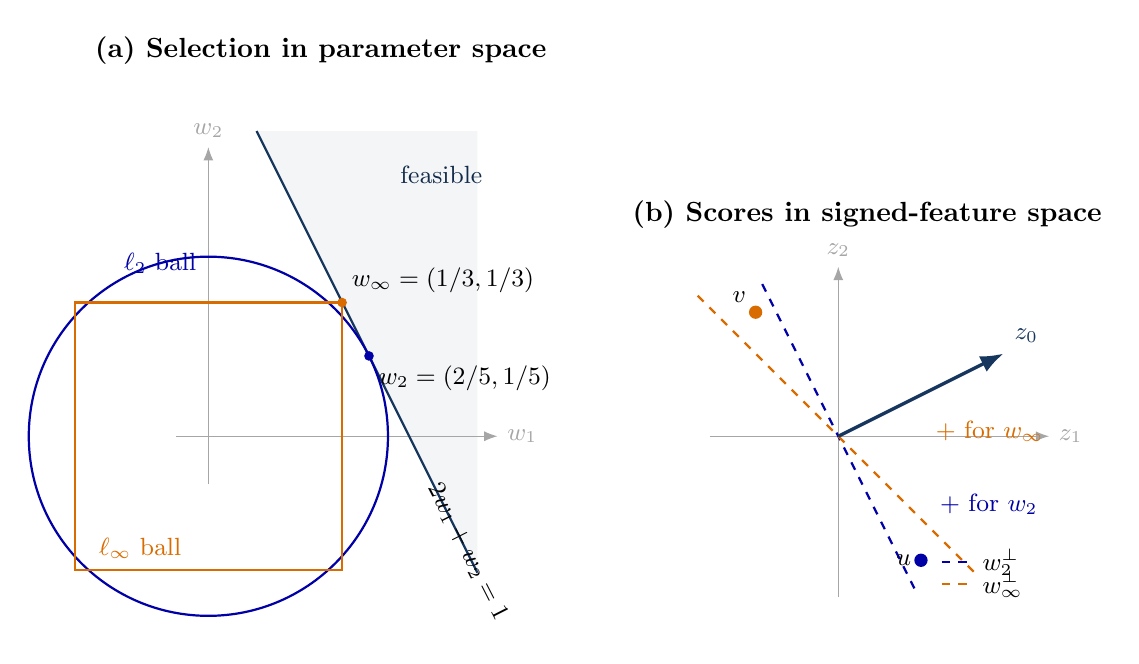
\begin{tikzpicture}[>=Latex,font=\small]
  \begin{scope}[x=5.1cm,y=5.1cm]
    \node[font=\bfseries] at (.28,.96) {(a) Selection in parameter space};
    \fill[courseblue!5] (.12,.76)--(.67,.76)--(.67,-.34)--cycle;
    \draw[->,gray!70] (-.08,0)--(.72,0) node[right] {$w_1$};
    \draw[->,gray!70] (0,-.12)--(0,.72) node[above] {$w_2$};
    \draw[thick,courseblue] (.12,.76)--(.67,-.34)
      node[pos=.78,right,black,rotate=-63] {$2w_1+w_2=1$};
    \draw[blue!65!black,thick] (0,0) circle ({sqrt(.2)});
    \draw[orange!85!black,thick]
      (-.333,-.333) rectangle (.333,.333);
    \fill[blue!65!black] (.4,.2) circle (.012)
      node[below right,black] {$w_2=(2/5,1/5)$};
    \fill[orange!85!black] (.333,.333) circle (.012)
      node[above right,black] {$w_\infty=(1/3,1/3)$};
    \node[blue!65!black] at (-.12,.43) {$\ell_2$ ball};
    \node[orange!85!black] at (-.17,-.28) {$\ell_\infty$ ball};
    \node[courseblue!80!black] at (.58,.65) {feasible};
  \end{scope}

  \begin{scope}[xshift=8.0cm,x=1.05cm,y=1.05cm]
    \node[font=\bfseries] at (.35,2.68) {(b) Scores in signed-feature space};
    \draw[->,gray!70] (-1.55,0)--(2.55,0) node[right] {$z_1$};
    \draw[->,gray!70] (0,-1.95)--(0,2.05) node[above] {$z_2$};
    \draw[dashed,blue!65!black,thick] (-.92,1.84)--(.92,-1.84);
    \draw[dashed,orange!85!black,thick] (-1.7,1.7)--(1.7,-1.7);
    \draw[->,very thick,courseblue] (0,0)--(2,1)
      node[above right] {$z_0$};
    \fill[blue!65!black] (1,-1.5) circle (2.4pt)
      node[left,black] {$u$};
    \fill[orange!85!black] (-1,1.5) circle (2.4pt)
      node[above left,black] {$v$};
    \node[blue!65!black] at (1.82,-.82) {$+$ for $w_2$};
    \node[orange!85!black] at (1.83,.06) {$+$ for $w_\infty$};
    \draw[dashed,blue!65!black,thick] (1.25,-1.52)--(1.62,-1.52)
      node[right,black] {$w_2^\perp$};
    \draw[dashed,orange!85!black,thick] (1.25,-1.79)--(1.62,-1.79)
      node[right,black] {$w_\infty^\perp$};
  \end{scope}
\end{tikzpicture}
\vspace{0.9em}

\begin{tabular}{c@{\qquad}cc}
\toprule
Signed feature & $\sign\langle w_2,z\rangle$
               & $\sign\langle w_\infty,z\rangle$\\
\midrule
$z_0=(2,1)$ & $+$ & $+$\\
$u=(1,-3/2)$ & $+$ & $-$\\
$v=(-1,3/2)$ & $-$ & $+$\\
\bottomrule
\end{tabular}
\caption{The same observed signed vector $z_0$ produces different
Euclidean and max-norm separators. Panel (a) shows the two norm balls at their
first contact with the hard-margin half-space. Panel (b) shows the resulting
decision boundaries. A population with rare point $u$ favors Euclidean
selection; replacing $u$ by $v$ favors max-norm selection.}
\label{fig:two-dimensional-reversal}
\end{figure}

The same example has a direct data-space interpretation. Regard $z_0$ as a
positive example and $-z_0$ as a negative example. Both produce the signed
feature $yx=z_0$, so both impose the same hard-margin constraint. Let
$H_w=\{x:\langle w,x\rangle=0\}$ and let $q$ be conjugate to $p$.
\begin{proposition}[Dual-norm distance to a hyperplane]
\label{prop:dual-distance-hyperplane}
Assume
$\langle w,z_0\rangle=1$. Then
\[
 \operatorname{dist}_q(z_0,H_w)
 =\frac{\langle w,z_0\rangle}{\|w\|_p}
 =\frac1{\|w\|_p}.
\]
\end{proposition}
\begin{proof}
For every $z\in H_w$, H\"older's inequality gives
\[
  1=\langle w,z_0-z\rangle
  \le \|w\|_p\|z_0-z\|_q.
\]
Hence $\operatorname{dist}_q(z_0,H_w)\ge 1/\|w\|_p$.
By norm duality, there exists $s$ with $\|s\|_q=1$ and
$\langle w,s\rangle=\|w\|_p$.  Setting
\[
  z=z_0-\frac{s}{\|w\|_p}
\]
gives $\langle w,z\rangle=1-1=0$, so $z\in H_w$, and
$\|z_0-z\|_q=1/\|w\|_p$. The matching upper bound proves equality.
\end{proof}
Thus minimizing the parameter norm $\|w\|_p$ maximizes the input-space margin
measured in the dual norm $\|\cdot\|_q$.

\Needspace{22\baselineskip}
\begin{figure}[H]
\centering
\vspace{0.5em}
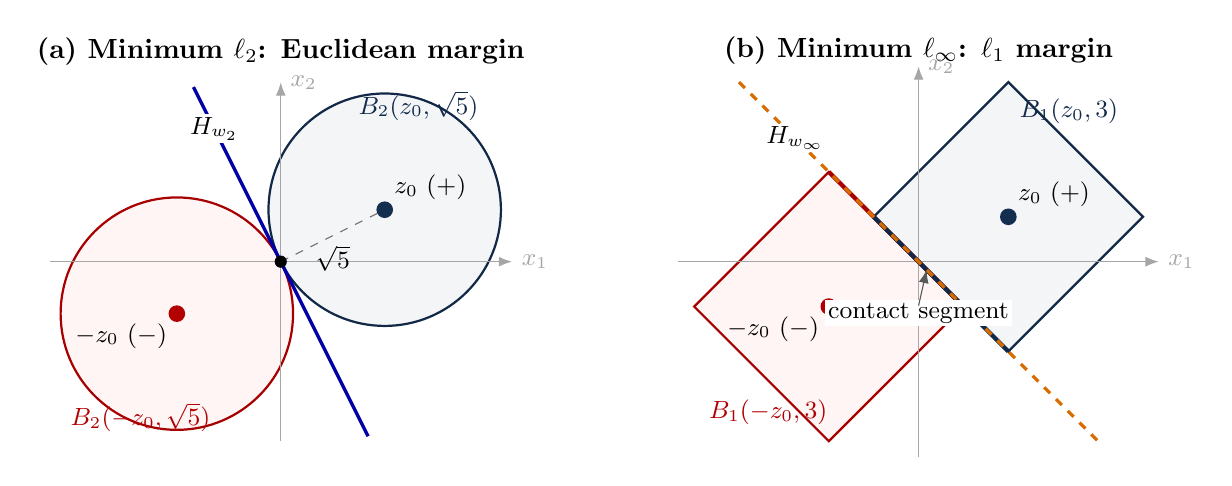
\begin{tikzpicture}[>=Latex,font=\small]
  \begin{scope}[x=.66cm,y=.66cm]
    \node[font=\bfseries] at (0,4.05)
      {(a) Minimum $\ell_2$: Euclidean margin};
    \draw[fill=red!4,draw=red!65!black,thick]
      (-2,-1) circle ({sqrt(5)});
    \draw[fill=courseblue!5,draw=courseblue!75!black,thick]
      (2,1) circle ({sqrt(5)});
    \draw[->,gray!70] (-4.45,0)--(4.45,0) node[right] {$x_1$};
    \draw[->,gray!70] (0,-3.45)--(0,3.45) node[right] {$x_2$};
    \draw[very thick,blue!65!black] (-1.68,3.36)--(1.68,-3.36);
    \node[fill=white,inner sep=1pt] at (-1.28,2.56) {$H_{w_2}$};
    \draw[dashed,black!55] (0,0)--(2,1)
      node[midway,below,black] {$\sqrt5$};
    \fill[black] (0,0) circle (2.2pt);
    \fill[courseblue!85!black] (2,1) circle (3pt)
      node[above right,black] {$z_0\ (+)$};
    \fill[red!70!black] (-2,-1) circle (3pt)
      node[below left,black] {$-z_0\ (-)$};
    \node[courseblue!80!black] at (2.65,3.0)
      {$B_2(z_0,\sqrt5)$};
    \node[red!70!black] at (-2.7,-3.0)
      {$B_2(-z_0,\sqrt5)$};
  \end{scope}

  \begin{scope}[xshift=8.1cm,x=.57cm,y=.57cm]
    \node[font=\bfseries] at (0,4.7)
      {(b) Minimum $\ell_\infty$: $\ell_1$ margin};
    \draw[fill=red!4,draw=red!65!black,thick]
      (-2,2)--(1,-1)--(-2,-4)--(-5,-1)--cycle;
    \draw[fill=courseblue!5,draw=courseblue!75!black,thick]
      (2,4)--(5,1)--(2,-2)--(-1,1)--cycle;
    \draw[->,gray!70] (-5.35,0)--(5.35,0) node[right] {$x_1$};
    \draw[->,gray!70] (0,-4.35)--(0,4.35) node[right] {$x_2$};
    \draw[line width=1.5pt,red!65!black] (-2,2)--(1,-1);
    \draw[line width=1.5pt,courseblue!75!black] (-1,1)--(2,-2);
    \draw[dashed,very thick,orange!85!black] (-4,4)--(4,-4);
    \node[fill=white,inner sep=1pt] at (-2.75,2.75) {$H_{w_\infty}$};
    \fill[courseblue!85!black] (2,1) circle (3pt)
      node[above right,black] {$z_0\ (+)$};
    \fill[red!70!black] (-2,-1) circle (3pt)
      node[below left,black] {$-z_0\ (-)$};
    \node[courseblue!80!black] at (3.35,3.35) {$B_1(z_0,3)$};
    \node[red!70!black] at (-3.35,-3.35) {$B_1(-z_0,3)$};
    \node[fill=white,inner sep=1pt] at (0,-1.15) {contact segment};
    \draw[->,black!65] (0,-.98)--(.18,-.18);
  \end{scope}
\end{tikzpicture}
\vspace{0.8em}
\caption{The two decision boundaries separate the positive point $z_0$ from
the negative point $-z_0$. The Euclidean separator $H_{w_2}$ supports
touching $\ell_2$ balls of radius $\sqrt5$. The max-norm separator
$H_{w_\infty}$ supports $\ell_1$ balls of radius $3$; because the $\ell_1$
ball is not strictly convex, contact occurs along line segments. The balls use
the input-space norm dual to the norm minimized in parameter space.}
\label{fig:two-dimensional-margin-balls}
\end{figure}

We now make the generalization comparison exact. Let $Y$ be uniform on
$\{-1,1\}$ and independent of a signed feature $Z$, and set $X=YZ$. Then
$YX=Z$. For $\delta\in(0,1)$, define two population laws:
\begin{align}
 P_2&:\quad \P(Z=z_0)=1-\delta,
                 &\P(Z=u)=\delta,\label{eq:p2-law}\\
 P_\infty&:\quad \P(Z=z_0)=1-\delta,
                 &\P(Z=v)=\delta.\label{eq:pinf-law}
\end{align}
Both laws are linearly separable at the population level: $(1,0)^\top$
separates the support of $P_2$, and $(0,1)^\top$ separates the support of
$P_\infty$.

For $p\in\{2,\infty\}$, let $\widehat w_p(S_n)$ be a minimum-$\ell_p$
solution of the empirical hard-margin constraints. For samples generated
by these laws, the solution is unique except when both support points appear;
when both points appear, any selected solution classifies both observed
support points correctly.

\begin{theorem}[Either norm-induced selector can have smaller expected population risk]
\label{thm:two-point-reversal}
For every $n\ge1$ and $\delta\in(0,1)$,
\begin{align*}
 \E_{P_2^n}\bigl[R_{P_2}(\widehat w_\infty(S_n))
               -R_{P_2}(\widehat w_2(S_n))\bigr]
 &=\delta(1-\delta)^n,\\
 \E_{P_\infty^n}\bigl[R_{P_\infty}(\widehat w_2(S_n))
               -R_{P_\infty}(\widehat w_\infty(S_n))\bigr]
 &=\delta(1-\delta)^n.
\end{align*}
The gap is maximized at $\delta=1/(n+1)$ and is asymptotic to $1/(en)$.
\end{theorem}

\begin{proof}
Let $E$ be the event that the common point $z_0$ is observed and the rare
point is absent. The two selectors can disagree in population risk only on
$E$, and $\P(E)=(1-\delta)^n$. Conditional on $E$,
\cref{prop:two-selectors} shows that the
disfavored selector misclassifies exactly the rare point, of population mass
$\delta$. If both support points appear, both empirical constraints enforce
correct classification of the entire support. If the sample contains only
the rare point, the two selectors have the same population risk. These cases prove
both identities.

For $g(\delta)=\delta(1-\delta)^n$,
\[
 g'(\delta)=(1-\delta)^{n-1}(1-(n+1)\delta),
\]
so the unique maximizer is $\delta=1/(n+1)$. At this value,
\[
 g(\delta)=\frac1{n+1}\left(\frac n{n+1}\right)^n
 \sim\frac1{en}.
\]
\end{proof}

This fixed two-dimensional construction makes the reversal transparent, but
its largest expected gap vanishes with $n$. The next result shows why the
effect can remain constant when the number of available features grows with
the sample size.

\section{A constant gap from private features}
\label{sec:amplification}

The two-dimensional example can be amplified without changing the global
norm or splitting optimization into separate tasks. Each signed feature vector
below has a two-dimensional shared block and an $n$-dimensional private block.
Rare identity $j$ activates only coordinate $j$ of the private feature block.
Training can therefore fit every observed identity by changing the
corresponding private parameter coefficient. For an unobserved identity, that
coefficient remains zero, so the shared block determines the prediction.

Fix the sample size $n\ge4$ and set $d=n+2$. Let
$e_1,\ldots,e_n$ be the standard basis of $\R^n$, and write a signed feature
as $(z^{\rm sh},z^{\rm pr})\in\R^2\times\R^n$. The common signed feature
vector is
\[
 z_0=((2,1)^\top,0).
\]
For each rare identity $j\in[n]$, define
\begin{align}
 u_j&=((1,-3/2)^\top,ne_j),
 \label{eq:rare-u}\\
 v_j&=((-1,3/2)^\top,ne_j).
 \label{eq:rare-v}
\end{align}
The two coordinate blocks have different purposes. The shared vectors
\[
 u=(1,-3/2)^\top,
 \qquad
 v=(-1,3/2)^\top=-u
\]
lie in the wedge between the two decision boundaries in
\cref{fig:two-dimensional-reversal}: the Euclidean and max-norm selectors
assign opposite signs to $u$, and their signs reverse at $v$. The first two
coordinates therefore determine how a selector extrapolates to an unseen
rare identity.

The basis vector $e_j$ specifies the private feature direction associated with
identity $j$. If identity $j$ is observed, its margin can be repaired by
changing only the corresponding private parameter coefficient. If identity
$j$ is absent, minimum-norm selection leaves that coefficient at zero, and the
prediction falls back to the shared two-dimensional score.
The factor $n$ makes the repair cheap: a constant margin deficit requires a
private coefficient of order $1/n$. Across at most $n$ observed identities,
the total squared Euclidean cost is therefore only $O(1/n)$, and the absolute
value of every private coefficient remains below the optimal max norm for
large $n$. Geometrically,
the construction consists of a common two-dimensional plane and one
orthogonal private direction for each rare identity.

Under $P_{2,n}$, the signed feature $Z$ takes the value $z_0$ with probability
$1/2$ and takes each value $u_j$ with probability $1/(2n)$. Under $P_{\infty,n}$,
$u_j$ is replaced by $v_j$. As before, draw an independent uniform label
$Y\in\{-1,1\}$ and set $X=YZ$. Both populations are linearly separable:
the parameter with shared block $(1,0)^\top$ and zero private block separates
$P_{2,n}$, while the parameter with shared block $(0,1)^\top$ and zero private
block separates $P_{\infty,n}$.

Let $\widehat w_2$ be the minimum-$\ell_2$ empirical hard-margin separator.
Let $\widehat w_\infty$ first minimize the global $\ell_\infty$ norm and then,
among those solutions, minimize the Euclidean norm. The Euclidean tie-break only
fixes otherwise irrelevant parameter coefficients. The tie-break agrees with
zero initialization on the coefficients associated with identities absent
from the sample.\endnote{The minimum-$\ell_\infty$
problem can have multiple solutions. The conclusions use only two properties
of the tie-break: a private parameter coefficient associated with an
unobserved identity remains zero, and no parameter coordinate exceeds the
optimal max norm. Zero-initialized coordinatewise methods have the first
property because no observed gradient has a component in that coordinate
direction.}

The event that at least one common example appears will be denoted by
\[
 G_n=\{z_0\text{ occurs in }S_n\}.
\]
The complement $G_n^c$ has probability $2^{-n}$.

\begin{lemma}[The shared parameter blocks retain the two-dimensional biases]
\label{lem:private-shared}
On $G_n$, the shared coordinates of $\widehat w_\infty$ equal
$(1/3,1/3)^\top$. The shared coordinates $\widehat w_2^{\rm sh}$ satisfy
\[
 \left\|\widehat w_2^{\rm sh}
       -\left(\frac25,\frac15\right)^\top\right\|_2^2
 \le \frac{121}{100n}.
\]
Every private parameter coefficient associated with an identity absent from
$S_n$ is zero for both selectors.
\end{lemma}

\begin{proof}
The common constraint is $2w_1+w_2\ge1$. Hence
$\|w\|_\infty\ge1/3$, with equality only if
$w_1=w_2=1/3$. For an observed $u_j$, the shared score of $u_j$ is
$-1/6$, and setting the corresponding private parameter coefficient to
$7/(6n)$ raises the margin to one. For an observed $v_j$, the required
coefficient is $5/(6n)$. These values are at most $1/3$ for $n\ge4$, so a
feasible separator with max norm $1/3$ exists. The shared coordinates of every
max-norm minimizer are therefore exactly $(1/3,1/3)^\top$. The Euclidean
tie-break sets every unused private parameter coefficient to zero.

For the Euclidean problem, write
$w_2^\star=(2/5,1/5)^\top$. A feasible comparison vector uses shared
coordinates $w_2^\star$ and, for every observed rare identity, a private
parameter coefficient $9/(10n)$ under $P_{2,n}$ or $11/(10n)$ under
$P_{\infty,n}$.
There are at most $n$ observed identities, so the squared norm of the
comparison vector is at most
\[
 \|w_2^\star\|_2^2+n\left(\frac{11}{10n}\right)^2
 =\frac15+\frac{121}{100n}.
\]
The common constraint and $w_2^\star=z_0^{\rm sh}/5$ imply, for every
feasible shared vector $a$,
\[
 \|a\|_2^2
 =\|w_2^\star\|_2^2
  +2\langle w_2^\star,a-w_2^\star\rangle
  +\|a-w_2^\star\|_2^2
 \ge\frac15+\|a-w_2^\star\|_2^2.
\]
The Euclidean minimizer has no larger norm than the comparison vector;
combining this comparison with the preceding inequality proves the
bound. Finally, an unused private parameter coefficient appears in no
constraint, so setting that coefficient to zero strictly decreases either
Euclidean norm used in the two selection rules unless the coefficient was
already zero.
\end{proof}

The Euclidean bound tends to zero. Since the shared Euclidean margins on
$(1,-3/2)^\top$ and $(-1,3/2)^\top$ are $1/10$ and $-1/10$, respectively,
the signs of these margins agree with the original two-dimensional example
for all
sufficiently large $n$.

\begin{theorem}[Global norm selection can differ by a constant in either direction]
\label{thm:private-amplification}
For the minimum-$\ell_2$ and minimum-$\ell_\infty$ selectors above,
\begin{align*}
 \E_{P_{2,n}^n}[R_{P_{2,n}}(\widehat w_2)]&\longrightarrow0,
 &
 \E_{P_{2,n}^n}[R_{P_{2,n}}(\widehat w_\infty)]
 &\longrightarrow\frac12e^{-1/2},\\
 \E_{P_{\infty,n}^n}[R_{P_{\infty,n}}(\widehat w_\infty)]&\longrightarrow0,
 &
 \E_{P_{\infty,n}^n}[R_{P_{\infty,n}}(\widehat w_2)]
 &\longrightarrow\frac12e^{-1/2}.
\end{align*}
Thus the limiting gap in either direction is approximately $0.303$.
\end{theorem}

\begin{proof}
On $G_n$, every observed rare identity is classified correctly because the
corresponding hard-margin constraint is present. For an unobserved rare
identity, the associated private parameter coefficient is zero by
\cref{lem:private-shared}. Under $P_{2,n}$, the Euclidean
shared score on every $u_j$ is positive for all sufficiently large $n$, while
the max-norm shared score is $-1/6$. Under $P_{\infty,n}$, the max-norm
shared score on every $v_j$ is $1/6$, while the Euclidean shared score is
negative for all sufficiently large $n$. The favored selector under each
population law therefore has
zero risk on $G_n$, and its expected risk is at most $\P(G_n^c)=2^{-n}$.

For a fixed rare identity $j$, the probability that it is absent while a
common point is present is
\[
 \left(1-\frac1{2n}\right)^n
 -\left(\frac12-\frac1{2n}\right)^n.
\]
Each rare signed-feature value has population mass $1/(2n)$. Summing over the
$n$ rare signed-feature values, the disfavored selector's expected error on
$G_n$ is
\begin{equation}
 \frac12\left[
 \left(1-\frac1{2n}\right)^n
 -\left(\frac12-\frac1{2n}\right)^n
 \right]\longrightarrow\frac12e^{-1/2}.
 \label{eq:private-unseen-mass}
\end{equation}
The contribution of $G_n^c$ is at most $2^{-n}$, proving all four limits.
\end{proof}

Here $d=n+2$, so the construction is in the proportional-dimensional,
slightly overparameterized regime. The construction is a sequence of problems
whose dimension and feature magnitudes grow with $n$. The theorem does not
establish inconsistency for one fixed finite-dimensional distribution.\endnote{The
nonzero entry in each
private feature block has magnitude $n$ so that fitting all observed private
identities changes the shared block of the minimum-Euclidean-norm separator by
only $O(n^{-1/2})$. The growing
scale is part of this exact construction and should not be hidden.}

The statistical mechanism is close to the example of \citet{wilson2017}.
There are recurring features that determine performance on new examples and
private features that permit the classifier to fit the training sample but do
not transfer to an unseen identity. The selected geometry determines how much
the fitted classifier relies on each kind of feature.

\section{Adam can move from max-norm to Euclidean bias}
\label{sec:adam}

For a gradient $g_t=\nabla L_n(w_t)$, bias-corrected Adam forms
coordinatewise exponential averages $\widehat m_t$ and $\widehat v_t$ of
$g_t$ and $g_t^2$, then updates
\begin{equation}
 w_{t+1}=w_t-\eta_t
 \frac{\widehat m_t}{\sqrt{\widehat v_t}+\epsilon}.
 \label{eq:adam}
\end{equation}
All operations in the fraction are coordinatewise. The positive stability
constant $\epsilon$ prevents division by zero.

When $\sqrt{\widehat v_t}$ dominates $\epsilon$ and the moving averages
track a nearly constant gradient direction, the denominator approximately
normalizes each coordinate and the update is sign-like. When the gradients
have become small relative to $\epsilon$, the denominator is approximately
constant and the update is gradient-like. These two limiting calculations
suggest two geometries, but the calculations do not by themselves determine
which parameter direction the entire trajectory approaches.

The following statement summarizes a recent result for deterministic,
full-batch, bias-corrected Adam on separable linear logistic classification.
The result uses polynomially decreasing stepsizes and fixed $\epsilon>0$,
together with regularity conditions ensuring the standard max-margin limits. The
comparison is made as $\epsilon\downarrow0$.

\begin{theorem}[Adam has early max-norm and late Euclidean regimes]
\label{thm:adam-two-regimes}
For sufficiently small fixed $\epsilon>0$, Adam reaches parameter vectors with
nearly optimal $\ell_\infty$ normalized margin before its updates become
gradient-like. At much later times its normalized parameter vector approaches
the minimum-$\ell_2$ hard-margin direction.
\end{theorem}

\begin{proof}[Proof outline]
When $\sqrt{\widehat v_t}\gg\epsilon$ coordinatewise, division by
$\sqrt{\widehat v_t}$ normalizes the gradient magnitudes. After controlling
the errors caused by the moving averages, the resulting update direction is a
perturbation of the signed-descent direction and inherits its $\ell_\infty$
max-margin behavior. The perturbation argument establishes a time interval on which the
normalized margin is arbitrarily close to the optimal $\ell_\infty$ margin as
$\epsilon\downarrow0$.

Because the data are separable, the logistic gradients vanish along the
trajectory. For every fixed $\epsilon>0$, eventually
$\sqrt{\widehat v_t}\ll\epsilon$. The denominator in \cref{eq:adam} is then
$\epsilon(1+o(1))$, and the first-moment average tracks the ordinary
gradient closely enough that Adam is an asymptotically vanishing perturbation
of Euclidean gradient descent. The Euclidean part of
\cref{thm:discrete-margin-selection} then gives the late minimum-$\ell_2$
direction.
The complete argument proves that the max-norm interval occurs before the
Euclidean asymptotic regime by bounding the two timescales uniformly in small
$\epsilon$.
\end{proof}

The point for this lecture is the distinction between the two selected
directions, not the detailed crossover. The normalized parameter vector can
remain close to the max-norm direction after the update has already become
gradient-like; the earlier updates have built a large component that later
updates must replace.\endnote{For stepsizes
$\eta_t\asymp(t+1)^{-a}$ with $1/3<a<1$, the submitted analysis places the
update crossover at a polylogarithmic scale in $1/\epsilon$, while reaching a
fixed Euclidean-margin accuracy requires a polynomial scale in
$1/\epsilon$. For $a=1$, the corresponding separation is polynomial versus
exponential. These rates are not needed for the risk examples in this
lecture.}

\begin{corollary}[The preferred checkpoint depends on the population law]
\label{cor:adam-risk}
In the two laws of \cref{thm:two-point-reversal}, a checkpoint whose parameter
direction is sufficiently close to the max-norm separator is preferred under
$P_\infty$, while a checkpoint sufficiently close to the Euclidean separator
is preferred under $P_2$.
\end{corollary}

\begin{proof}
For each sample-support pattern in the two-point construction, the relevant
Euclidean and max-norm separators assign nonzero scores to both population
support points. Classification risk is therefore constant in a sufficiently
small neighborhood of each separator. Apply \cref{thm:adam-two-regimes} to
choose an early checkpoint in the max-norm neighborhood and a late checkpoint
in the Euclidean neighborhood. The expected-risk identities in
\cref{thm:two-point-reversal} then give the two stated preferences.
\end{proof}

The corollary conditionally transfers the two-selector calculation; the
corollary is not an exact finite-time risk formula for Adam. The conclusion
is that stopping later can
improve or worsen population classification even after the training sample
has become perfectly classified. The sign of the change depends on the
population law.

The practical response is to retain checkpoints and select among them using
held-out data. Validation does not identify a universally correct optimizer;
validation tests which point on the realized trajectory predicts better for the
available validation distribution.

There is no conflict with the construction of \citet{wilson2017}. Their
published exact example concerns least-squares classification and idealized
adaptive methods whose denominator has no fixed positive stability constant.
With $\epsilon=0$, coordinate normalization can persist forever. With fixed
$\epsilon>0$, the denominator eventually stops normalizing vanishing
gradients, which permits the late Euclidean regime in separable logistic
classification. In least squares, moreover, an early adaptive update can
create a null-space component. Later ordinary gradients lie in the data row
space and cannot remove that component.

\section{Stepsize schedules determine whether noise persists}
\label{sec:stepsize-noise}

The word ``stochastic'' does not by itself determine the long-run behavior of
an optimization method. The stepsize schedule determines whether successive
perturbations become negligible or continue to accumulate. The following
one-dimensional calculation gives the basic distinction exactly.

Fix $\mu>0$ and consider the quadratic objective
$L(\theta)=\mu\theta^2/2$. Let $\Xi_1,\Xi_2,\ldots$ be independent random
variables with mean zero and variance $\sigma^2>0$. Starting from a fixed
$\theta_0$, use the unbiased stochastic gradient $\mu\Theta_t+\Xi_{t+1}$:
\begin{equation}
 \Theta_{t+1}
 =\Theta_t-\eta_t(\mu\Theta_t+\Xi_{t+1}).
 \label{eq:noisy-quadratic}
\end{equation}

\begin{proposition}[Constant-stepsize iterates fluctuate; decreasing-stepsize iterates converge]
\label{prop:constant-decreasing-step}
For the recursion in \cref{eq:noisy-quadratic}:
\begin{enumerate}[(a),leftmargin=*]
\item If $\eta_t=\eta\in(0,2/\mu)$, then
\[
 \E[\Theta_t]\longrightarrow0,
 \qquad
 \operatorname{Var}(\Theta_t)\longrightarrow
 \frac{\eta\sigma^2}{\mu(2-\mu\eta)}>0.
\]
\item If $\eta_t=1/(\mu(t+1))$, then, for every $t\ge1$,
\[
 \Theta_t=-\frac1{\mu t}\sum_{s=1}^t\Xi_s,
 \qquad
 \E[\Theta_t^2]=\frac{\sigma^2}{\mu^2t}.
\]
Consequently, $\Theta_t\to0$ in mean square and almost surely.
\end{enumerate}
\end{proposition}

\begin{proof}
For a constant stepsize, set $a=1-\mu\eta$, so $|a|<1$. Independence and
zero mean give
\[
 \E[\Theta_{t+1}]=a\E[\Theta_t],
 \qquad
 \operatorname{Var}(\Theta_{t+1})
 =a^2\operatorname{Var}(\Theta_t)+\eta^2\sigma^2.
\]
The variance recursion converges to
$\eta^2\sigma^2/(1-a^2)=\eta\sigma^2/[\mu(2-\mu\eta)]$.
For the decreasing schedule, induction in \cref{eq:noisy-quadratic} gives the
displayed empirical average. Its second moment is
$\sigma^2/(\mu^2t)$, and almost-sure convergence follows from the strong law
of large numbers.
\end{proof}

Under a constant stepsize, the distribution of the iterate retains nonzero
spread around the unique minimizer; the iterate does not approach the
minimizer itself. The limiting standard deviation is of order $\sqrt{\eta}$.
A smaller constant stepsize reduces this spread but does not remove the
asymptotic fluctuation. The decreasing schedule eventually suppresses the
noise.

The general stochastic-approximation conditions
\begin{equation}
 \sum_{t=0}^\infty\eta_t=\infty,
 \qquad
 \sum_{t=0}^\infty\eta_t^2<\infty
 \label{eq:robbins-monro-steps}
\end{equation}
express the same balance. The first sum leaves enough cumulative movement to
reach a solution; the second makes the cumulative variance of bounded
mean-zero perturbations finite. Additional assumptions are needed for a
general convergence theorem, especially for a nonconvex objective.

Constant stepsize has a different effect when the set of minimizers contains a
curve or manifold with tangent directions along which there is no restoring
gradient. After $t$ independent mean-zero increments of size $\eta$, the
accumulated displacement has standard deviation of order $\eta\sqrt{t}$.
The resulting variance accumulation is \emph{diffusive behavior}: order-one motion
along a flat solution set occurs on the timescale $t\asymp\eta^{-2}$.
State-dependent noise can also create a systematic drift along the flat solution set and
thereby prefer some solutions to others. At an isolated unique minimizer,
the same noise instead produces a stationary distribution concentrated near
that point.

There is an important exception. Constant stepsize does not create persistent
motion when the stochastic gradient noise itself vanishes at every exact fit.
For squared-loss prediction, let
\[
 \ell_i(\theta)=\frac12\bigl(f_\theta(x_i)-y_i\bigr)^2.
\]

\begin{proposition}[Interpolation can remove minibatch noise]
\label{prop:interpolation-removes-noise}
If $f_\theta(x_i)=y_i$ for every training example, then every per-example and
minibatch gradient is zero at $\theta$.
\end{proposition}

\begin{proof}
For every $i$,
\[
 \nabla\ell_i(\theta)
 =\bigl(f_\theta(x_i)-y_i\bigr)\nabla f_\theta(x_i)=0.
\]
Every minibatch gradient is an average of these vectors.
\end{proof}

This proposition explains why minibatch SGD and gradient descent have the
same minimum-norm bias in interpolating linear least squares. In a nonconvex
network, minibatch noise may still change the basin reached before
interpolation, but the minibatch noise stops once every individual residual is
zero. Continued motion along a zero-loss set requires nonvanishing noise, such
as fresh label perturbations, or another mechanism that prevents every
individual gradient from vanishing.

The disappearance of minibatch noise differs from a common
stochastic-approximation model in engineering, in
which every gradient query contains fresh measurement or simulation noise
whose variance remains positive at a minimizer. Minibatch noise from a fixed
finite empirical objective is state dependent. Whether noise persists at a
solution is therefore a property of the loss, data, and noise mechanism, not
an automatic consequence of using a stochastic update.

Practical schedules often use long constant-stepsize phases followed by one
or more reductions. During a constant phase, persistent noise can explore or
move along a set of low-loss parameters. Reducing the stepsize concentrates
the iterates and can eventually fix one of those parameters. A stepsize
reduction can change population performance only when the points visited by
the dynamics define different predictors or extrapolate differently;
stochasticity alone gives no ordering of their population risks.

\section{What the examples establish}
\label{sec:scope}

Does the direction selected by the optimizer matter? Yes, when the empirical
constraints leave predictions on unobserved inputs undetermined. The
two-dimensional example gives an exact order-$1/n$ effect, and the
proportional-dimensional example gives a constant effect. Neither direction
is universally better. The examples and the noisy-quadratic calculation
support four specific conclusions.

First, the empirical objective need not determine the returned predictor.
In least squares, initialization fixes the component orthogonal to the data
span. In separable logistic classification, the update geometry fixes a
limiting margin geometry.

Second, an optimizer-induced preference is not automatically a statistically
correct preference. Euclidean and max-norm selection each win on one of the
two population laws. A norm can be useful only relative to structure in the
data-generating law, such as which features or contexts recur at test time.

Third, growing dimension can change the magnitude of the effect. The
two-dimensional ambiguity occurs only when one rare point is missing, giving
an order-$1/n$ maximal expected gap. With $\Theta(n)$ rare identities, a
constant fraction of population mass can belong to identities absent from the
sample, giving a constant gap.

Fourth, the stepsize schedule determines the asymptotic role of gradient
noise. Decreasing stepsizes can permit convergence by making the cumulative
noise variance finite. A constant stepsize with persistent noise produces a
stationary fluctuation near an isolated solution or diffusive motion along a
solution set. If every stochastic gradient vanishes at interpolation, even a
constant stepsize supplies no continuing noise.

The linear setting isolates optimizer-induced selection exactly. The linear
analysis does not describe feature learning in a deep network and does not
imply that Adam or SGD is uniformly preferable in applications. Empirical
comparisons have found both
meaningful optimizer-dependent gaps and substantial dependence on tuning,
architecture, and task. The theorem-level conclusion is the absence of a
universal ordering.

\section{Optional reading\suppmark}
\label{sec:optional}

\subsection{Early stopping induces a spectral filter}
\label{sec:spectral-filter}

Return to least squares with $w_0=0$. Set
$H=\mathbf X^\top\mathbf X$ and $b=\mathbf X^\top y$. Suppose
$0<\eta<2/\|H\|_{\mathrm{op}}$, and write
\[
 H=\sum_{j=1}^d\lambda_jq_jq_j^\top
\]
for an orthonormal eigenbasis, with $\lambda_j\ge0$.

\begin{proposition}[Finite-time gradient descent filters eigendirections]
\label{prop:spectral-filter}
For every $t\ge1$,
\[
 w_t=\sum_{j:\lambda_j>0}
 \frac{1-(1-\eta\lambda_j)^t}{\lambda_j}
 \langle q_j,b\rangle q_j.
\]
\end{proposition}

\begin{proof}
The update is $w_{t+1}=(I-\eta H)w_t+\eta b$. Since $w_0=0$, unrolling the
recurrence gives
\[
 w_t=\eta\sum_{k=0}^{t-1}(I-\eta H)^k b.
\]
Moreover, $b=\mathbf X^\top y$ is orthogonal to $\ker H$. Along the
eigendirection spanned by $q_j$ with $\lambda_j>0$, the coefficient is
therefore
\[
 \eta\sum_{k=0}^{t-1}(1-\eta\lambda_j)^k\langle q_j,b\rangle
 =\frac{1-(1-\eta\lambda_j)^t}{\lambda_j}
  \langle q_j,b\rangle.
\]
Summing these coefficients proves the formula.
\end{proof}

The scalar function
\[
 g_t(\lambda)=\frac{1-(1-\eta\lambda)^t}{\lambda}
\]
is a \emph{spectral filter}: the function $g_t$ specifies how strongly the
procedure responds to the data in each eigendirection of $H$. At convergence,
$g_\infty(\lambda)=1/\lambda$. At finite time, if
$\eta t\lambda\ll1$, then $g_t(\lambda)\approx\eta t$. Thus early stopping
does not yet apply the large inverse factor $1/\lambda$ to directions with
small eigenvalues. The transition occurs around
$\lambda\approx1/(\eta t)$. Ridge regression uses the related filter
$g_\rho(\lambda)=1/(\lambda+\rho)$.

The filter formula explains why a stopping time can act as regularization even
before considering different limiting optima: the stopping time changes which
spectral components have had time to enter the solution.
\Cref{ex:l10-spectral-filter} asks you to derive
the formula and compare the two filters.

\subsection{The Wilson construction}
\label{sec:wilson}

The least-squares construction of \citet{wilson2017} uses one feature
coordinate that reveals the label, two constant feature coordinates, and many
feature coordinates that are nonzero in only one training example.
Zero-initialized gradient methods remain
in the row span and reach the minimum-$\ell_2$ interpolant. In their example,
the minimum-$\ell_2$ classifier uses the recurring label feature and has
asymptotically zero classification error. AdaGrad, RMSProp, and Adam without
a positive stability offset follow a coordinate-normalized ray that assigns
the same parameter-coordinate magnitude to private and recurring features;
the resulting
classifier predicts the majority class on new examples and can have error
arbitrarily close to $1/2$. A finite version uses $O(n)$ features.

Their exact ray calculation is not specific to squared loss. Let
$\mathbf X$ have row $i$ equal to $x_i^\top$, let $y\in\{-1,1\}^n$, set
$s=\sign(\mathbf X^\top y)$, and suppose
\begin{equation}
 \mathbf Xs=cy
 \label{eq:equal-margin-ray}
\end{equation}
for some $c>0$.

\begin{proposition}[Equal margins preserve the signed-gradient ray]
\label{prop:equal-margin-ray}
For any differentiable margin loss
$L(w)=\sum_{i=1}^n\ell(y_i\langle w,x_i\rangle)$ and every $\alpha\ge0$,
\[
 \nabla L(\alpha s)=\ell'(c\alpha)\mathbf X^\top y.
\]
If $\ell'<0$, signed gradient descent initialized at zero remains on the ray
$\{\alpha s:\alpha\ge0\}$.
\end{proposition}

\begin{proof}
Equation \cref{eq:equal-margin-ray} gives
$y_i\langle s,x_i\rangle=c$ for every $i$. Hence
\[
 \nabla L(\alpha s)
 =\sum_{i=1}^n\ell'(c\alpha)y_ix_i
 =\ell'(c\alpha)\mathbf X^\top y.
\]
Since $s=\sign(\mathbf X^\top y)$ and $\ell'<0$, the negative signed
gradient is $s$ on every nonzero coordinate. Induction proves the ray claim.
\end{proof}

Logistic loss satisfies the proposition, so the equal-margin ray remains
invariant for logistic loss when the adaptive denominator exactly cancels
coordinate magnitudes. The proposition does not extend the published
population theorem to ordinary Adam with fixed $\epsilon>0$: the added
$\epsilon$ breaks exact
coordinate cancellation as gradients vanish. \Cref{ex:l10-equal-margin-ray}
asks you to verify both the margin-loss and squared-loss calculations.

\subsection{Noisy selection in neural networks and flatness}
\label{sec:noise-flatness}

\Cref{prop:interpolation-removes-noise} shows that ordinary minibatch noise
vanishes at squared-loss interpolation. A clean way to keep stochasticity
active is to perturb the label afresh at every update. Consider
\[
 L(\theta)=\frac1{2n}\sum_{i=1}^n
 \bigl(f_\theta(x_i)-y_i\bigr)^2
\]
and its zero-training-error set
\[
 \mathcal M=\{\theta:f_\theta(x_i)=y_i\text{ for every }i\}.
\]
At an update using example $i$, replace $y_i$ by $y_i+\Xi$, where $\Xi$ has
mean zero and variance $\sigma^2$ and is sampled independently at each step.
At $\theta\in\mathcal M$, the gradient contribution is
$-\Xi\nabla f_\theta(x_i)$, so its covariance depends on the network
Jacobians. The corresponding scalar quantity is
\begin{equation}
 \mathcal R(\theta)
 =\frac1n\sum_{i=1}^n\|\nabla f_\theta(x_i)\|_2^2
 =\operatorname{tr}\bigl(\nabla^2L(\theta)\bigr),
 \qquad \theta\in\mathcal M.
 \label{eq:label-noise-regularizer}
\end{equation}
The equality uses the zero residuals: the residual-weighted second-derivative
terms in the Hessian vanish on $\mathcal M$.

The next statement summarizes a local small-stepsize result for smooth
networks with bounded derivatives and independent bounded label noise of
constant variance. The setup is deliberately different from ordinary
minibatch SGD on an exactly interpolated dataset.

\begin{theorem}[Label-noise dynamics select minimizers of a Jacobian regularizer]
\label{thm:label-noise-regularizer}
A zero-training-error parameter is locally attractive for the label-noise
training dynamics precisely when it is a local minimizer of
$\mathcal R$ restricted to the zero-error manifold $\mathcal M$.
\end{theorem}

\begin{proof}[Proof outline]
Near $\mathcal M$, decompose a parameter displacement into components normal
and tangent to the manifold. The squared-loss Hessian contracts the normal
component. Fresh label perturbations keep producing normal fluctuations, so
for a small constant stepsize this fast component approaches a local
Ornstein--Uhlenbeck-type equilibrium rather than vanishing.

A second-order expansion of the update, averaged over these fast
fluctuations, produces a slower tangential drift. Its leading term is a
vector proportional to
\[
 -P_{T_\theta\mathcal M}\nabla\mathcal R(\theta),
\]
where $P_{T_\theta\mathcal M}$ is the orthogonal projection operator onto the
tangent space of $\mathcal M$. Thus the averaged slow dynamics descend the
restriction of
$\mathcal R$ to $\mathcal M$. Under the stated smoothness and boundedness
assumptions, the higher-order terms are uniformly smaller for a sufficiently
small stepsize. The locally attractive zero-error parameters are therefore
exactly the constrained local minima of $\mathcal R$. The cited paper gives
the perturbation bounds that justify the fast--slow averaging.
\end{proof}

The theorem is a genuine optimizer-induced selection result for neural
networks of arbitrary smooth architecture. The label-noise dynamics have two
timescales: the loss first becomes
small, and the persistent noise then produces much slower motion within
$\mathcal M$. A more general diffusion analysis describes the slow motion by
a stochastic differential equation on the solution manifold. Both the drift
and the covariance of this stochastic differential equation depend on the
loss and on the covariance of the injected
noise. Isotropic noise, label noise, and minibatch noise therefore need not
select the same parameters.

The theorem does not say that minimizing $\mathcal R$ always improves
population risk. An improvement in population risk requires an additional
argument connecting
the Jacobian regularizer to the data-generating law. Such a connection has
been proved in some simplified nonlinear models, but not for arbitrary deep
networks.

The label-noise result also gives a precise sense in which noise can prefer
``flatter'' parameters, but the result does not validate an unspecified
flat-minimum principle.
For a ReLU unit,
\begin{equation}
 a\,[b^\top x]_+
 =\frac ac\,[(cb)^\top x]_+,
 \qquad c>0.
 \label{eq:relu-rescaling}
\end{equation}
The two parameter vectors define the same predictor, but raw Hessian
eigenvalues and parameter-space neighborhood volumes can change under the
rescaling. Consequently, parameter-space sharpness is not by itself a
function of the learned predictor and cannot by itself explain a difference
in population risk. The parameterization dependence does not rule out every invariant or
algorithm-relative notion of flatness. The rescaling example rules out
treating an arbitrary raw Hessian measure as a parameterization-independent
explanation. In
\cref{thm:label-noise-regularizer}, the parameterization-dependent quantity is
meaningful because $\mathcal R$ is derived from a specified update rule and noise model.

\section{Take-home messages}
\label{sec:take-home}

\begin{itemize}[leftmargin=*]
\item A decreasing stepsize can suppress stochastic-gradient noise and permit
convergence. A constant stepsize with persistent noise instead produces a
stationary fluctuation near an isolated minimizer or diffusive motion along a
solution set. Constant stepsize alone is insufficient: at squared-loss
interpolation, ordinary minibatch noise vanishes.
\item The empirical objective may leave the predictor underdetermined.
Initialization and update geometry then complete the selection rule: zero-initialized
least-squares gradient descent selects the minimum-$\ell_2$ interpolant, while
different steepest-descent geometries select different max-margin directions.
\item Minimum-$\ell_2$ and minimum-$\ell_\infty$ selection can have opposite
population-risk orderings. The data-generating law, not the empirical fit
alone, determines which extrapolation is useful.
\item A fixed two-dimensional problem gives an order-$1/n$ expected gap. With
$\Theta(n)$ private features, the gap can approach
$e^{-1/2}/2\approx0.303$. Adam can move
from the max-norm geometry toward the Euclidean geometry, so an early or late
checkpoint can be preferable depending on the population.
\end{itemize}

\clearpage
\printendnotes

\section*{Bibliographical notes}

The Euclidean max-margin limit of discrete gradient descent on separable
logistic regression is due to \citet{soudry2018}. The treatment of implicit
bias in terms of mirror-descent and steepest-descent geometry, including
general norms, follows \citet{gunasekar2018}. The discrete normalized
steepest-descent and signed-gradient result stated in
\cref{thm:discrete-margin-selection} follows the analysis of
\citet{fan2025spectral}; its decreasing-stepsize assumptions should not be
replaced by a generic appeal to the continuous-time limit. \citet{balles2018}
explain the relation between sign-based updates and steepest descent in max
norm.

The examples in \cref{sec:two-dimensional,sec:amplification} were developed
for these notes to make the population-risk reversal explicit in both
directions. The private-feature construction is inspired by the use of many
example-specific features in \citet{wilson2017}; no priority claim is made
for the construction. Wilson et al. give a squared-loss example in which
standard gradient methods generalize well and AdaGrad, RMSProp, and Adam can
approach chance error. They also report optimizer-dependent differences on
CIFAR-10 and language tasks. Later benchmark studies, including
\citet{sivaprasad2020}, emphasize that such comparisons depend strongly on
tuning and experimental protocol.

The separability and steepest-direction diagrams were typeset by Diego Gomez
from the pictures used in class.

The two-regime Adam statement summarizes \citet{fan2026}. Its endpoint
results build on
\citet{wang2022,zhang2024}: zero-offset Adam has max-norm margin bias, whereas
fixed-positive-offset Adam eventually has Euclidean margin bias. Related
work studies how optimizer geometry interacts with modern architectures and
feature structure; examples include \citet{schmidt2021,zhang2024transformers}
and \citet{vasudeva2025}.

The stepsize calculation in \cref{prop:constant-decreasing-step} is an
elementary instance of classical stochastic approximation. The local
stationary-distribution view of constant-stepsize SGD is developed by
\citet{mandt2017}. The label-noise characterization in
\cref{thm:label-noise-regularizer} is due to \citet{blanc2020};
\citet{li2022} give a general diffusion framework for motion near a smooth
manifold of minimizers. Complete statistical comparisons are known in simpler
nonlinear parameterizations. For example, \citet{haochen2021} show that the
noise covariance changes sparse recovery in a quadratically parameterized
model, and \citet{pesme2021} compare stochastic and deterministic gradient
flows in diagonal linear networks. These results support a
noise-model-dependent selection principle, not a universal advantage for
SGD.

The spectral-filter view of iterative regularization is classical; see
\citet{yao2007}. The caution about parameter-space sharpness and the ReLU
rescaling example follow \citet{dinh2017}. Flatness can still enter valid
generalization analyses after the relevant parameterization, perturbation,
or invariant quantity is specified; the objection is to an unqualified raw
Hessian explanation.

\section*{Glossary}

\begin{description}[style=nextline,leftmargin=1.5em,labelindent=0pt]
\item[Algorithmic bias]
In this lecture, the preference among empirical solutions or limiting
directions induced by an optimization algorithm. We use the term only in
this optimization sense.
\item[Explicit regularization]
Adding or imposing an auxiliary criterion that prefers some empirical
solutions, such as a norm penalty or constraint.
\item[Diffusive behavior]
Accumulation of persistent mean-zero perturbations whose variance grows
proportionally to time in directions without a restoring gradient.
\item[Gradient noise]
The difference between a stochastic gradient and the corresponding full
empirical gradient. Its magnitude and covariance can depend on the current
parameter.
\item[Implicit bias]
The preference among empirical solutions or limiting directions induced by
the initialization, update geometry, or stopping rule while the empirical
objective is fixed.
\item[Logit]
A real-valued score interpreted as log-odds. In binary logistic regression,
$\langle w,x\rangle=\log(q_w(1\mid x)/q_w(-1\mid x))$.
\item[Linearly separable sample]
A labeled sample for which one linear score has strictly positive signed
margin on every observed example.
\item[Margin]
The signed score $y\langle w,x\rangle$; after normalization by a norm of $w$,
the resulting normalized margin is invariant to positive rescaling of the
parameter vector $w$.
\item[Margin loss]
A training loss $\ell(y s(x))$ that depends on a labeled example through its
signed margin.
\item[Model non-uniqueness]
The existence of empirically optimal parameters that represent different
predictors on at least one input.
\item[Normalized empirical margin]
The smallest signed score on the training sample divided by a specified norm
of the parameter. The normalized empirical margin depends only on the
direction of a nonzero parameter vector.
\item[Max-margin separator]
A parameter direction that separates the sample and maximizes the smallest
normalized empirical margin. Equivalently, it is the direction of a
minimum-norm vector satisfying unit hard-margin constraints.
\item[Overparameterized]
A regime in which the parameterization has more degrees of freedom than the
observed constraints need, so many exact empirical fits can exist.
\item[Parameter-space non-uniqueness]
The existence of distinct empirically optimal parameter vectors, possibly
representing the same predictor.
\item[Strictly proper scoring rule]
A probability-prediction loss whose conditional expected value is uniquely
minimized by reporting the true conditional distribution.
\item[Regularizer]
An auxiliary parameter- or predictor-dependent criterion used to prefer some
fits to others.
\item[Spectral filter]
A scalar response function that specifies how a linear estimator weights
each eigendirection of a data-dependent matrix.
\item[Steepest descent]
An optimization method that chooses the direction of greatest local decrease
measured in a specified norm. Changing the norm changes the update geometry.
\item[Surrogate loss]
A tractable training loss used in place of the deployment loss that directly
defines the task evaluation.
\end{description}

\section{Exercises}
\label{sec:exercises}

\exerciseinstructions
\setcounter{courseexercise}{0}
\begin{exercisechunk}
\item \textbf{Initialization and the minimum-norm least-squares solution.}
\label[exercise]{ex:l10-least-squares-selection}
\exerciseprofile{2}{2}{2}{\exproof\quad\excalculation}{%
Identify the invariant component of least-squares gradient descent and derive
the solution selected by its initialization.}
Fix $x_1,\ldots,x_n\in\R^d$ and $y_1,\ldots,y_n\in\R$. Let
\[
 \cR=\operatorname{span}\{x_1,\ldots,x_n\},
 \qquad \dim(\cR)=n,
\]
let $\mathbf X\in\R^{n\times d}$ have row $i$ equal to $x_i^\top$, and set
$y=(y_1,\ldots,y_n)^\top$. Define
\[
 L_n(w)=\frac12\sum_{i=1}^n
 \bigl(\langle w,x_i\rangle-y_i\bigr)^2.
\]
Consider gradient descent
\[
 w_{t+1}=w_t-
 \eta\sum_{i=1}^n
 \bigl(\langle w_t,x_i\rangle-y_i\bigr)x_i,
 \qquad 0<\eta<2/\|\mathbf X\|_{\mathrm{op}}^2.
\]
\begin{enumerate}[(a),beginpenalty=10000]
\item Derive the normal equation in both forms
\[
 \sum_{i=1}^n
 \bigl(\langle w,x_i\rangle-y_i\bigr)x_i=0,
 \qquad
 \mathbf X^\top(\mathbf Xw-y)=0.
\]
Prove that $\dim(\cR)=n$ is equivalent to
$\mathbf X\mathbf X^\top$ being nonsingular, and deduce that the normal
equation is equivalent to $\mathbf Xw=y$.

\item Define
$w^\star=\mathbf X^\top(\mathbf X\mathbf X^\top)^{-1}y$.
Prove that every minimizer of $L_n$ has the unique form
\[
 w^\star+v,
 \qquad v\in\cR^\perp.
\]
Use the Pythagorean theorem to prove that $w^\star$ is the unique
minimum-Euclidean-norm minimizer.

\item Let $v_0$ be the orthogonal projection of $w_0$ onto $\cR^\perp$.
Prove that the $\cR^\perp$ component of every iterate equals $v_0$ and that
\[
 w_t\longrightarrow w^\star+v_0.
\]
Deduce the limit for $w_0=0$, and give an initialization whose limit is not
the minimum-norm minimizer.
\end{enumerate}
\begin{hints}
For (a), use the rank of $\mathbf X$ and the fact that a full-column-rank
matrix $\mathbf X^\top$ is one-to-one. For (b), first substitute $w^\star$
into $\mathbf Xw=y$. For (c), every increment belongs to $\cR$; on $\cR$, use
an eigenbasis of $\mathbf X^\top\mathbf X$.
\end{hints}
\end{exercisechunk}

\begin{exercisechunk}
\item \textbf{Logits, sigmoid probabilities, and logistic loss.}
\label[exercise]{ex:l10-logistic-log-loss}
\exerciseprofile{2}{2}{2}{\exproof\quad\excalculation\quad\exinterpretation}{%
Derive binary logistic loss from a conditional probability model and
distinguish the probabilistic surrogate from classification error.}
Define the sigmoid function by
\[
 \sigma(s)=\frac1{1+e^{-s}},
 \qquad s\in\R.
\]
For a score $s_w(x)=\langle w,x\rangle$ and a label
$y\in\{-1,1\}$, define
\[
 q_w(y\mid x)=\sigma\bigl(ys_w(x)\bigr).
\]
Lecture~1 introduced a binary logit as log-odds, and Lecture~3 introduced
sigmoid probabilities and log-loss fitting. This exercise reconnects those
ideas for a linear score.
\begin{enumerate}[(a),beginpenalty=10000]
\item Prove that $\sigma(s)+\sigma(-s)=1$. Deduce that
$q_w(\cdot\mid x)$ is a probability mass function on $\{-1,1\}$ for every
$x$.

\item Prove the log-odds identity
\[
 \log\frac{q_w(1\mid x)}{q_w(-1\mid x)}=s_w(x),
\]
and derive
\[
 -\log q_w(y\mid x)
 =\log\bigl(1+e^{-ys_w(x)}\bigr).
\]
Use these identities to explain each part of the terminology: why $s_w(x)$ is
a \emph{logit}, why the use of $\sigma$ makes the model \emph{logistic}, why
modeling $\P(Y=1\mid X=x)$ as a function of $x$ is called \emph{regression},
and why the negative log-likelihood is called \emph{logistic loss}.

\item Fix an input $x$ and suppose
$\pi=\P(Y=1\mid X=x)\in(0,1)$. If a predictor assigns probability
$q\in(0,1)$ to label $1$, its conditional expected log loss is
\[
 C_\pi(q)=-\pi\log q-(1-\pi)\log(1-q).
\]
Prove that $C_\pi$ is uniquely minimized at $q=\pi$. State precisely what the
identity $q=\pi$ implies when the logistic model can represent the true
conditional probabilities.

\item Show that $q_w(1\mid x)\ge1/2$ if and only if $s_w(x)\ge0$.
Compare the logistic training loss with the deployment loss
$\I\{\operatorname{sign}(s_w(x))\ne y\}$. Why is logistic loss called a
surrogate loss for classification error?
\end{enumerate}
\begin{hints}
For (c), differentiate $C_\pi(q)$ and determine the sign of its derivative
on either side of $q=\pi$. For (d), the two losses use the same signed score,
but one records its magnitude and the other records only whether its sign is
correct.
\end{hints}
\end{exercisechunk}

\begin{exercisechunk}
\item \textbf{Why steepest-descent flow escapes to infinity.}
\label[exercise]{ex:l10-flow-escape}
\exerciseprofile{2}{2}{2}{\exproof\quad\excalculation}{%
Complete the descent argument that makes separable logistic loss vanish along
unit steepest-descent flow.}
Fix a linearly separable collection $z_1,\ldots,z_n\in\R^d$, let
\[
 L_n(w)=\frac1n\sum_{i=1}^n\log(1+e^{-\langle w,z_i\rangle}),
\]
and let $w(t)$ solve the unit steepest-descent flow
\[
 \dot w(t)=s_p(\nabla L_n(w(t))).
\]
Let $q$ be conjugate to $p$, let $\gamma_p^\star>0$ be the maximum
normalized margin, and define
\[
 a_i(t)=\frac1{n(1+e^{\langle w(t),z_i\rangle})},
 \qquad A(t)=\sum_{i=1}^n a_i(t).
\]
Set $L_0=L_n(w(0))$.
\begin{enumerate}[(a),beginpenalty=10000]
\item Prove
\[
 \|\nabla L_n(w(t))\|_q\ge\gamma_p^\star A(t)
\]
and
\[
 -\frac{d}{dt}L_n(w(t))=\|\nabla L_n(w(t))\|_q.
\]

\item Prove that $L_n(w(t))\le L_0$ and that
\[
 A(t)\ge e^{-nL_0}L_n(w(t)).
\]

\item Deduce the explicit bound
\[
 L_n(w(t))
 \le L_0\exp\bigl(-\gamma_p^\star e^{-nL_0}t\bigr).
\]
Conclude that every margin $\langle w(t),z_i\rangle$ tends to infinity and
that $\|w(t)\|_p\to\infty$.
\end{enumerate}
\begin{hints}
For (b), put $x_i=e^{-\langle w(t),z_i\rangle}$. Use
$x_i\ge\log(1+x_i)$ and
$\log(1+x_i)\le nL_n(w(t))\le nL_0$.
For (c), apply the differential inequality from parts (a)--(b), then use the
fact that the loss is a finite sum of nonnegative terms.
\end{hints}
\end{exercisechunk}

\begin{exercisechunk}
\item \textbf{Complete the max-margin flow proof.}
\label[exercise]{ex:l10-flow-proof-details}
\exerciseprofile{3}{2}{3}{\exproof\quad\excalculation}{%
Supply the finite-sum and limiting arguments used in the max-margin flow
proof.}
Fix linearly separable vectors $z_1,\ldots,z_n\in\R^d$ and let
\[
 L_n(w)=\frac1n\sum_{i=1}^n\log(1+e^{-\langle w,z_i\rangle}).
\]
Let $w(t)$ be a trajectory such that $L_n(w(t))\to0$ and
$\|w(t)\|_p\to\infty$. Write
\[
 m_i(t)=\langle w(t),z_i\rangle,\quad
 m_{\min}(t)=\min_{i\in[n]}m_i(t),\quad
 a_i(t)=\frac1{n(1+e^{m_i(t)})},\quad
 A(t)=\sum_{i=1}^n a_i(t).
\]
\begin{enumerate}[(a),beginpenalty=10000]
\item Derive
\[
 \nabla L_n(w(t))=-\frac1n\sum_{i=1}^n\frac{z_i}{1+e^{m_i(t)}}
 =-\sum_{i=1}^n a_i(t)z_i.
\]

\item Prove that every $m_i(t)\to\infty$ and that
\[
 \frac{A(t)}{L_n(w(t))}\longrightarrow1.
\]

\item Prove that, for all sufficiently large $t$,
\[
 m_{\min}(t)\le-\log L_n(w(t))
 \le m_{\min}(t)+\log(2n).
\]
Conclude that
\[
 -\log L_n(w(t))=m_{\min}(t)+O(1).
\]

\item Suppose that for every $\varepsilon\in(0,\gamma_p^\star)$ and all
sufficiently large $t$,
\[
 -\frac{d}{dt}\log L_n(w(t))
 \ge(\gamma_p^\star-\varepsilon)\frac{d}{dt}\|w(t)\|_p.
\]
Integrate this inequality and use part (c) to prove
\[
 \gamma_p(w(t))\longrightarrow\gamma_p^\star.
\]

\item Suppose $w(t_k)/\|w(t_k)\|_p\to u$. Prove that
$\|u\|_p=1$ and
\[
 \min_i\langle u,z_i\rangle=\gamma_p^\star.
\]
Show that $u/\gamma_p^\star$ solves
\[
 \min_w\|w\|_p
 \quad\text{subject to}\quad
 \langle w,z_i\rangle\ge1\quad(i\in[n]).
\]
\end{enumerate}
\begin{hints}
For (b), use the corresponding scalar asymptotic equivalence for each of the
finitely many summands. For (c), use
$x/2\le\log(1+x)\le x$ for $x\in[0,1]$.
For (e), compare an arbitrary feasible vector with its normalized direction.
\end{hints}
\end{exercisechunk}

\begin{exercisechunk}
\item \textbf{The discrete steepest-descent estimate.}\suppmark
\label[exercise]{ex:l10-discrete-steepest}
\exerciseprofile{3}{2}{3}{\exproof\quad\excalculation\quad\exinterpretation}{%
Prove a discrete margin estimate and distinguish unit and scaled
steepest-descent stepsizes.}
Fix linearly separable vectors $z_1,\ldots,z_n\in\R^d$, let
\[
 L_n(w)=\frac1n\sum_{i=1}^n\log(1+e^{-\langle w,z_i\rangle}),
 \qquad
 \gamma_p^\star
 =\max_{\|u\|_p\le1}\min_{i\in[n]}\langle u,z_i\rangle,
\]
and let $q$ be conjugate to $p$. For $g\ne0$, choose
\[
 s_p(g)\in\operatorname*{arg\,min}_{\|v\|_p=1}\langle g,v\rangle,
\]
so that
$\|s_p(g)\|_p=1$ and
$\langle-g,s_p(g)\rangle=\|g\|_q$.
Suppose that $L_n$ is $B$-smooth relative to $\|\cdot\|_p$: for all
$w,\Delta$,
\[
 L_n(w+\Delta)
 \le L_n(w)+\langle\nabla L_n(w),\Delta\rangle
       +\frac B2\|\Delta\|_p^2.
\]
Consider the scaled discrete update
\[
 w_{t+1}=w_t+\eta_t\|g_t\|_q s_p(g_t),
 \qquad g_t=\nabla L_n(w_t).
\]
Assume $\eta_t\to0$, $L_n(w_t)\to0$, and
\[
 \sum_{t=0}^\infty\eta_t\|g_t\|_q=\infty.
\]
\begin{enumerate}[(a),beginpenalty=10000]
\item Prove the one-step inequalities
\begin{align*}
 L_n(w_{t+1})
 &\le L_n(w_t)-\eta_t\|g_t\|_q^2
       +\frac B2\eta_t^2\|g_t\|_q^2,\\
 \|w_{t+1}\|_p-\|w_t\|_p
 &\le\eta_t\|g_t\|_q.
\end{align*}

\item Define
\[
 A_t=\frac1n\sum_{i=1}^n
 \frac1{1+e^{\langle w_t,z_i\rangle}}.
\]
Prove that
\[
 \frac{A_t}{L_n(w_t)}\longrightarrow1
 \quad\text{and}\quad
 \|g_t\|_q\ge\gamma_p^\star A_t.
\]
Deduce that for every $\varepsilon>0$ and all sufficiently large $t$,
\[
 \log\frac{L_n(w_t)}{L_n(w_{t+1})}
 \ge(\gamma_p^\star-\varepsilon)
       \eta_t\|g_t\|_q.
\]

\item Sum the inequalities from parts (a)--(b) and prove
\[
 \gamma_p(w_t)\longrightarrow\gamma_p^\star.
\]

\item A unit-direction update has the form
\[
 w_{t+1}=w_t+\alpha_t s_p(g_t).
\]
Show that the unit-direction update equals the scaled update in this exercise
exactly when
$\alpha_t=\eta_t\|g_t\|_q$. Deduce the following translations:
\begin{enumerate}[(i)]
\item gradient descent with multiplier $\beta_t$ is represented by $p=2$,
$\eta_t=\beta_t$, and unit-direction length
$\alpha_t=\beta_t\|g_t\|_2$;
\item signed gradient descent with multiplier $\beta_t$ is represented by $p=\infty$,
$\alpha_t=\beta_t$, and scaled multiplier
$\eta_t=\beta_t/\|g_t\|_1$ whenever $g_t\ne0$.
\end{enumerate}
Explain why a stepsize theorem for the scaled update cannot be applied to
signed gradient descent without checking the transformed multipliers.
\end{enumerate}
\begin{hints}
For (b), use $-\log(1-x)\ge x$ after applying the one-step loss bound, and
use $\eta_t\to0$ to absorb the quadratic term. For (c), compare both
$-\log L_n(w_t)$ and $\|w_t\|_p$ with
$\sum_{s<t}\eta_s\|g_s\|_q$; then use
$-\log L_n(w_t)=\min_i\langle w_t,z_i\rangle+O(1)$.
\end{hints}
\end{exercisechunk}

\begin{exercisechunk}
\item \textbf{A two-point population-risk reversal.}
\label[exercise]{ex:l10-two-point-reversal}
\exerciseprofile{2}{2}{2}{\exproof\quad\excalculation\quad\exinterpretation}{%
Compute two norm-induced separators and relate their disagreement to expected
population classification risk.}
Let
\[
 z_0=(2,1)^\top,
 \qquad u=(1,-3/2)^\top,
 \qquad v=(-1,3/2)^\top.
\]
For $p\in\{2,\infty\}$, let $\widehat w_p$ minimize $\|w\|_p$ subject to
the hard-margin constraints in an observed sample.
\begin{enumerate}[(a),beginpenalty=10000]
\item When every observed signed feature equals $z_0$, derive
\[
 \widehat w_2=(2/5,1/5)^\top,
 \qquad
 \widehat w_\infty=(1/3,1/3)^\top.
\]
Determine the sign of the score assigned by each vector to $u$ and to $v$.

\item Fix $\delta\in(0,1)$. Under $P_2$, let $Z=z_0$ with probability
$1-\delta$ and $Z=u$ with probability $\delta$. Under $P_\infty$, replace
$u$ by $v$. In either law, draw $Y$ uniformly from $\{-1,1\}$ independently
of $Z$ and set $X=YZ$. For an i.i.d. sample $S_n$, prove
\begin{align*}
 \E_{P_2^n}[R_{P_2}(\widehat w_2)]&=0,&
 \E_{P_2^n}[R_{P_2}(\widehat w_\infty)]
 &=\delta(1-\delta)^n,\\
 \E_{P_\infty^n}[R_{P_\infty}(\widehat w_\infty)]
 &=(1-\delta)\delta^n,&
 \E_{P_\infty^n}[R_{P_\infty}(\widehat w_2)]
 &=\delta(1-\delta)^n+(1-\delta)\delta^n.
\end{align*}

\item Maximize the risk difference over $\delta$ and determine its asymptotic
order as $n\to\infty$. Explain in one sentence why the calculation gives no
universal population-risk ordering of the two norm biases.
\end{enumerate}
\begin{hints}
For (b), partition the samples into those containing only the common point,
only the rare point, or both. A hard-margin solution classifies every support
point that appears in its constraints.
\end{hints}
\end{exercisechunk}

\begin{exercisechunk}
\item \textbf{A constant gap from private features.}
\label[exercise]{ex:l10-private-features}
\exerciseprofile{3}{3}{3}{\exproof\quad\excalculation\quad\exinterpretation}{%
Prove that unseen private features amplify a two-dimensional norm bias into a
constant expected-risk gap in proportional dimension.}
Fix $n\ge4$, set $d=n+2$, and decompose
$z=(z^{\rm sh},z^{\rm pr})\in\R^2\times\R^n$. Define
\[
 z_0=((2,1)^\top,0),\quad
 u_j=((1,-3/2)^\top,ne_j),\quad
 v_j=((-1,3/2)^\top,ne_j),\quad j\in[n].
\]
Under $P_{2,n}$, $Z=z_0$ with probability $1/2$ and
$Z=u_j$ with probability $1/(2n)$ for every $j$. Under $P_{\infty,n}$,
replace $u_j$ by $v_j$. Draw $Y$ uniformly and independently from
$\{-1,1\}$ and set $X=YZ$. Let $S_n$ be an i.i.d. sample.

Let $\widehat w_2$ be the minimum-$\ell_2$ hard-margin separator. Let
$\widehat w_\infty$ minimize the global $\ell_\infty$ norm and then minimize
the Euclidean norm among the max-norm minimizers. Let
$G_n=\{z_0\text{ appears in }S_n\}$.
\begin{enumerate}[(a),beginpenalty=10000]
\item Prove that on $G_n$ the shared coordinates of
$\widehat w_\infty$ equal $(1/3,1/3)^\top$. Exhibit feasible private parameter
coefficients for every observed rare identity under each population, and prove
that the coefficient associated with every unobserved identity is zero.

\item Set $w_2^\star=(2/5,1/5)^\top$. Construct a feasible Euclidean
comparison vector and prove that, on $G_n$,
\[
 \|\widehat w_2^{\rm sh}-w_2^\star\|_2^2
 \le\frac{121}{100n}.
\]
Deduce that the signs assigned by the shared coordinates to the rare points
agree with those in the two-dimensional example for all sufficiently large
$n$.

\item For a fixed rare identity $j$, compute the probability that $j$ is
absent from $S_n$ while $G_n$ occurs. Sum over $j$ and prove that the favored
selector has expected risk tending to zero while the disfavored selector has
expected risk tending to
\[
 \frac12e^{-1/2}.
\]
Prove this conclusion under both $P_{2,n}$ and $P_{\infty,n}$, with the roles
of the selectors reversed.

\item State precisely which aspects of the learning problem change with
$n$. Does the result prove inconsistency for a fixed finite-dimensional
population law?
\end{enumerate}
\begin{hints}
For (a), the common constraint and $\|w\|_\infty\le1/3$ force equality in
$2w_1+w_2\le3\|w\|_\infty$. For (b), use at most $n$ private parameter
coefficients, each of magnitude at most $11/(10n)$. For (c), subtract the
event that neither
the common point nor identity $j$ appears from the event that identity $j$
does not appear.
\end{hints}
\end{exercisechunk}

\begin{exercisechunk}
\item \textbf{Equal margins preserve a signed-gradient ray.}\suppmark
\label[exercise]{ex:l10-equal-margin-ray}
\exerciseprofile{2}{2}{2}{\exproof\quad\excalculation\quad\exinterpretation}{%
Recognize when coordinate normalization confines an adaptive method to one
parameter ray.}
Let $\mathbf X\in\R^{n\times d}$ have row $i$ equal to $x_i^\top$, let
$y\in\{-1,1\}^n$, and define
\[
 s=\operatorname{sign}(\mathbf X^\top y).
\]
Assume $\mathbf Xs=cy$ for some $c>0$.
\begin{enumerate}[(a),beginpenalty=10000]
\item For a differentiable margin loss
$L(w)=\sum_{i=1}^n\ell(y_i\langle w,x_i\rangle)$, prove that
\[
 \nabla L(\alpha s)=\ell'(c\alpha)\mathbf X^\top y.
\]
When $\ell'<0$, prove by induction that signed gradient descent initialized
at zero remains on the ray $\{\alpha s:\alpha\ge0\}$.

\item For the squared loss
$Q(w)=\frac12\|\mathbf Xw-y\|_2^2$, prove
\[
 \nabla Q(\alpha s)=(c\alpha-1)\mathbf X^\top y.
\]
Explain why an adaptive update that divides each nonzero gradient coordinate
by a matching coordinatewise magnitude also remains on the ray.

\item Explain why replacing the denominator $|g_j|$ by $|g_j|+\epsilon$ for
fixed $\epsilon>0$ generally breaks the exact ray calculation as the gradient
vanishes. Contrast the consequences for a finite least-squares interpolant
and for logistic loss on separable data.
\end{enumerate}
\end{exercisechunk}

\begin{exercisechunk}
\item \textbf{Early stopping as a spectral filter.}\suppmark
\label[exercise]{ex:l10-spectral-filter}
\exerciseprofile{2}{2}{2}{\exproof\quad\excalculation\quad\exinterpretation}{%
Diagonalize least-squares gradient descent and interpret stopping time as
eigendirection-dependent regularization.}
Let $H=\mathbf X^\top\mathbf X$, $b=\mathbf X^\top y$, $w_0=0$, and
\[
 w_{t+1}=(I-\eta H)w_t+\eta b,
 \qquad 0<\eta<2/\|H\|_{\mathrm{op}}.
\]
Let $H=\sum_{j=1}^d\lambda_jq_jq_j^\top$ be an orthonormal
eigendecomposition.
\begin{enumerate}[(a),beginpenalty=10000]
\item Prove that
\[
 w_t=\sum_{j:\lambda_j>0}
 \frac{1-(1-\eta\lambda_j)^t}{\lambda_j}
 \langle q_j,b\rangle q_j.
\]
Justify why the coordinates with $\lambda_j=0$ vanish.

\item Define
$g_t(\lambda)=[1-(1-\eta\lambda)^t]/\lambda$. Show that
$g_t(\lambda)\to1/\lambda$ for every positive eigenvalue. For
$0\le\eta\lambda\le1$, prove
\[
 1-e^{-\eta\lambda t}
 \le 1-(1-\eta\lambda)^t
 \le \eta\lambda t.
\]
Use these bounds to identify the transition scale in $\lambda$.

\item Ridge regression uses the filter
$g_\rho(\lambda)=1/(\lambda+\rho)$. Compare the limiting behavior of
$g_t$ and $g_\rho$ when $\lambda$ is much larger or much smaller than
$1/(\eta t)$ and $\rho$, respectively. State the sense in which early
stopping regularizes small-eigenvalue directions.
\end{enumerate}
\begin{hints}
For (a), unroll the affine recursion and sum a geometric series in each
eigendirection. For (b), use $1-x\le e^{-x}$ and Bernoulli's inequality.
\end{hints}
\end{exercisechunk}


\clearpage
\setlength{\bibsep}{4pt}
\begin{thebibliography}{99}

\bibitem[Balles and Hennig(2018)]{balles2018}
Lukas Balles and Philipp Hennig.
\newblock Dissecting Adam: The sign, magnitude and variance of stochastic
gradients.
\newblock Proceedings of the 35th International Conference on Machine
Learning, 2018.
\newblock \url{https://proceedings.mlr.press/v80/balles18a.html}.

\bibitem[Blanc et al.(2020)]{blanc2020}
Guy Blanc, Neha Gupta, Gregory Valiant, and Paul Valiant.
\newblock Implicit regularization for deep neural networks driven by an
Ornstein--Uhlenbeck like process.
\newblock Proceedings of the 33rd Conference on Learning Theory, 2020.
\newblock \url{https://proceedings.mlr.press/v125/blanc20a.html}.

\bibitem[Dinh et al.(2017)]{dinh2017}
Laurent Dinh, Razvan Pascanu, Samy Bengio, and Yoshua Bengio.
\newblock Sharp minima can generalize for deep nets.
\newblock Proceedings of the 34th International Conference on Machine
Learning, 2017.
\newblock \url{https://proceedings.mlr.press/v70/dinh17b.html}.

\bibitem[Gunasekar et al.(2018)]{gunasekar2018}
Suriya Gunasekar, Jason D. Lee, Daniel Soudry, and Nathan Srebro.
\newblock Characterizing implicit bias in terms of optimization geometry.
\newblock Proceedings of the 35th International Conference on Machine
Learning, 2018.
\newblock \url{https://proceedings.mlr.press/v80/gunasekar18a.html}.

\bibitem[HaoChen et al.(2021)]{haochen2021}
Jeff Z. HaoChen, Colin Wei, Jason D. Lee, and Tengyu Ma.
\newblock Shape matters: Understanding the implicit bias of the noise
covariance.
\newblock Proceedings of the 34th Conference on Learning Theory, 2021.
\newblock \url{https://proceedings.mlr.press/v134/haochen21a.html}.

\bibitem[Fan and Szepesv\'ari(2026)]{fan2026}
Chen Fan and Csaba Szepesv\'ari.
\newblock On the two faces of Adam in separable linear classification.
\newblock arXiv preprint arXiv:2609.33904, 2026.
\newblock \url{https://arxiv.org/abs/2609.33904}.

\bibitem[Fan et al.(2025)]{fan2025spectral}
Chen Fan, Mark Schmidt, and Christos Thrampoulidis.
\newblock Implicit bias of spectral descent and Muon on multiclass separable
data.
\newblock Advances in Neural Information Processing Systems, 38, 2025.
\newblock \url{https://arxiv.org/abs/2502.04664}.

\bibitem[Li et al.(2022)]{li2022}
Zhiyuan Li, Tianhao Wang, and Sanjeev Arora.
\newblock What happens after SGD reaches zero loss?---A mathematical
framework.
\newblock International Conference on Learning Representations, 2022.
\newblock \url{https://openreview.net/forum?id=siCt4xZn5Ve}.

\bibitem[Mandt et al.(2017)]{mandt2017}
Stephan Mandt, Matthew D. Hoffman, and David M. Blei.
\newblock Stochastic gradient descent as approximate Bayesian inference.
\newblock Journal of Machine Learning Research, 18(134):1--35, 2017.
\newblock \url{https://www.jmlr.org/papers/v18/17-214.html}.

\bibitem[Pesme et al.(2021)]{pesme2021}
Scott Pesme, Loucas Pillaud-Vivien, and Nicolas Flammarion.
\newblock Implicit bias of SGD for diagonal linear networks: A provable
benefit of stochasticity.
\newblock Advances in Neural Information Processing Systems, 34, 2021.
\newblock \url{https://proceedings.neurips.cc/paper/2021/hash/f4661398cb1a3abd3ffe58600bf11322-Abstract.html}.

\bibitem[Schmidt et al.(2021)]{schmidt2021}
Robin M. Schmidt, Frank Schneider, and Philipp Hennig.
\newblock Descending through a crowded valley---benchmarking deep learning
optimizers.
\newblock Proceedings of the 38th International Conference on Machine
Learning, 2021.
\newblock \url{https://proceedings.mlr.press/v139/schmidt21a.html}.

\bibitem[Sivaprasad et al.(2020)]{sivaprasad2020}
Prabhu Teja Sivaprasad, Florian Mai, Thijs Vogels, Martin Jaggi, and
Fran\c{c}ois Fleuret.
\newblock Optimizer benchmarking needs to account for hyperparameter tuning.
\newblock Proceedings of the 37th International Conference on Machine
Learning, 2020.
\newblock \url{https://proceedings.mlr.press/v119/sivaprasad20a.html}.

\bibitem[Soudry et al.(2018)]{soudry2018}
Daniel Soudry, Elad Hoffer, Mor Shpigel Nacson, Suriya Gunasekar, and
Nathan Srebro.
\newblock The implicit bias of gradient descent on separable data.
\newblock Journal of Machine Learning Research, 19(70):1--57, 2018.
\newblock \url{https://www.jmlr.org/papers/v19/18-188.html}.

\bibitem[Vasudeva et al.(2025)]{vasudeva2025}
Bhavya Vasudeva, Jung Whan Lee, Vatsal Sharan, and Mahdi Soltanolkotabi.
\newblock The rich and the simple: On the implicit bias of Adam and SGD.
\newblock Advances in Neural Information Processing Systems, 38, 2025.
\newblock \url{https://arxiv.org/abs/2505.24022}.

\bibitem[Wang et al.(2022)]{wang2022}
Bohan Wang, Qi Meng, Huishuai Zhang, Ruoyu Sun, Wei Chen, Zhi-Ming Ma, and
Tie-Yan Liu.
\newblock Does momentum change the implicit regularization on separable data?
\newblock Advances in Neural Information Processing Systems, 2022.

\bibitem[Wilson et al.(2017)]{wilson2017}
Ashia C. Wilson, Rebecca Roelofs, Mitchell Stern, Nathan Srebro, and
Benjamin Recht.
\newblock The marginal value of adaptive gradient methods in machine
learning.
\newblock Advances in Neural Information Processing Systems, 30, 2017.
\newblock \url{https://papers.nips.cc/paper_files/paper/2017/hash/81b3833e2504647f9d794f7d7b9bf341-Abstract.html}.

\bibitem[Yao et al.(2007)]{yao2007}
Yuan Yao, Lorenzo Rosasco, and Andrea Caponnetto.
\newblock On early stopping in gradient descent learning.
\newblock Constructive Approximation, 26:289--315, 2007.

\bibitem[Zhang et al.(2024a)]{zhang2024}
Chenyang Zhang, Difan Zou, and Yuan Cao.
\newblock The implicit bias of Adam on separable data.
\newblock Advances in Neural Information Processing Systems, 37, 2024.

\bibitem[Zhang et al.(2024b)]{zhang2024transformers}
Yushun Zhang, Congliang Chen, Tian Ding, Ziniu Li, Ruoyu Sun, and
Zhi-Quan Luo.
\newblock Why transformers need Adam: A Hessian perspective.
\newblock Advances in Neural Information Processing Systems, 37, 2024.

\end{thebibliography}

\end{document}
